%%%%%%%%%%%%%%%%%%%%%%%%%%%%%%%%%%%%%%%%%%%%%%%%
%% Compile the master file!
%% 		Slides: Stefan Müller
%% 		Course: GK Linguistik
%%%%%%%%%%%%%%%%%%%%%%%%%%%%%%%%%%%%%%%%%%%%%%%%

%% -*- coding:utf-8 -*-

\iftoggle{ba-linguistik}{
\title{Grundkurs Linguistik}

\subtitle{Syntax}

\author{
	{Stefan Müller}
%	\\
%	{\footnotesize \url{http://www.linguistik.hu-berlin.de/staff/amyp}\\
%	\href{mailto:mapriema@hu-berlin.de}{mapriema@hu-berlin.de}}
}

\institute{Institut für deutsche Sprache und Linguistik}

%%%%%%%%%%%%%%%%%%%%%%%%%      
\date{ }
%\publishers{\textbf{6. linguistischer Methodenworkshop \\ Humboldt-Universität zu Berlin}}

%\hyphenation{nobreak}


%%%%%%%%%%%%%%%%%%%%%%%%%%%%%%%%%%%%%%%%%%%%%%%%%%%%
%%%             Preamble's End                   %%%
%%%%%%%%%%%%%%%%%%%%%%%%%%%%%%%%%%%%%%%%%%%%%%%%%%%%      


\huberlintitlepage[22pt]
}

\section{Syntax}
\author{Stefan Müller}


\iftoggle{ba-linguistik}{




\frame{
\frametitle{Lach Dich schlapp!}

\vfill

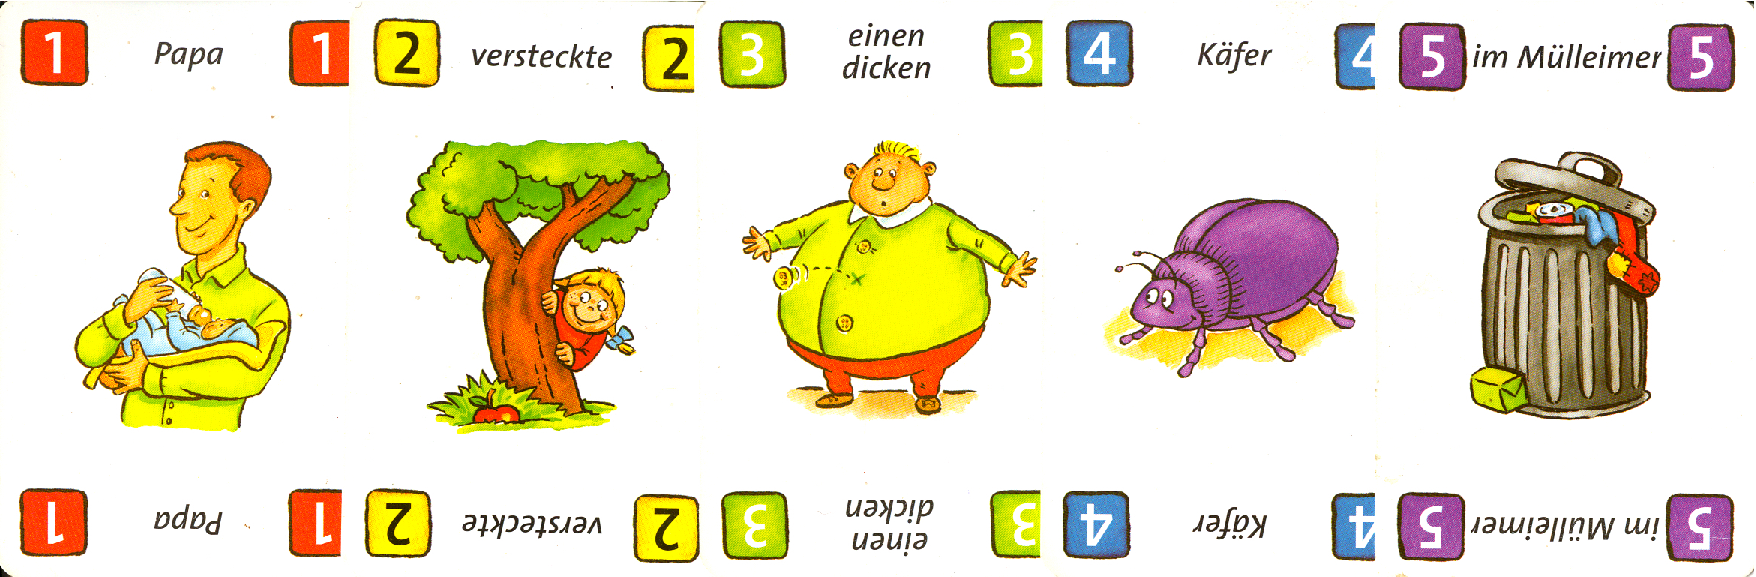
\includegraphics[width=\textwidth]{Bilder/lach-dich-schlapp-pappa-versteckte}

\vfill
Reihe die Spielkarten in der Reihenfolge 1 bis 5 aneinander.

\vfill
\footnotesize{(Ravensburger, 6--12 Jahre)}

}
\frame{
\frametitle{Lach Dich schlapp!}

\vfill
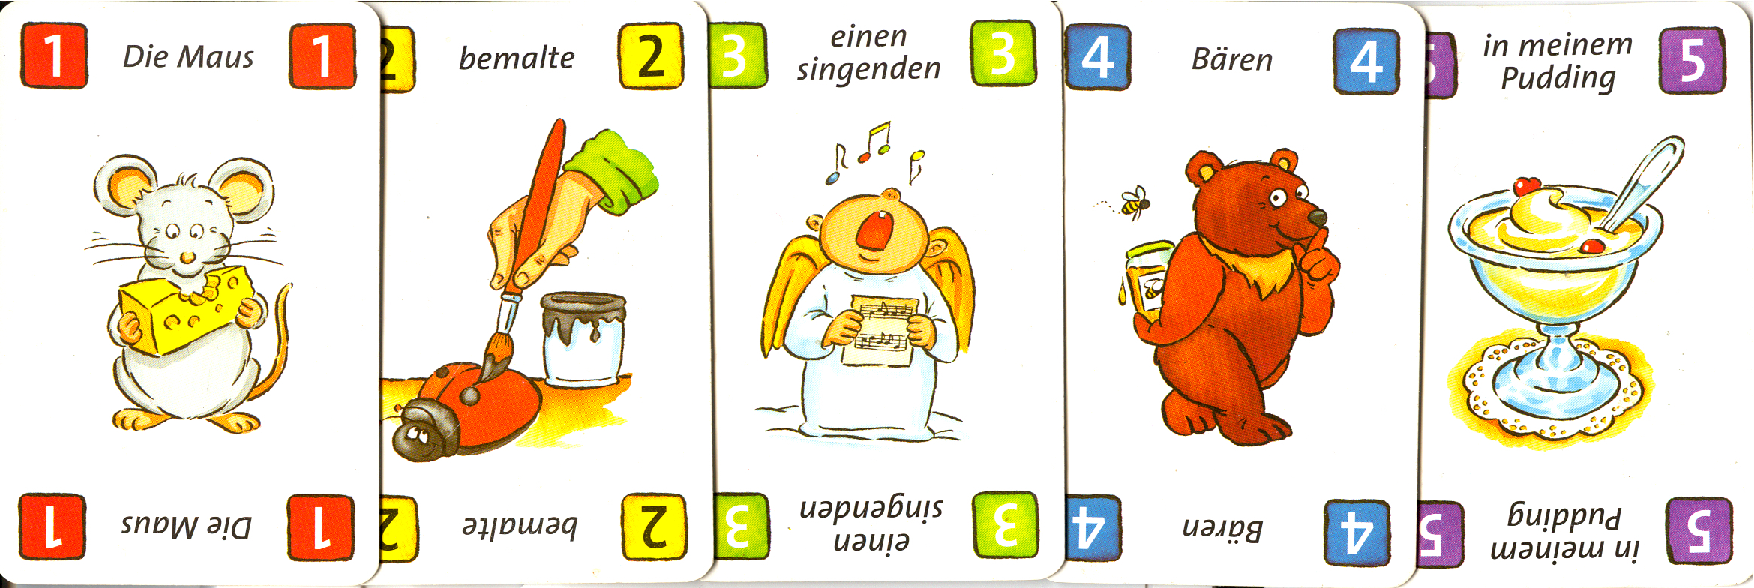
\includegraphics[width=\textwidth]{Bilder/lach-dich-schlapp-die-maus-bemalte}

\vfill
Warum funktioniert das Spiel?

\vfill
}


\frame{
\frametitle{Form und Bedeutung}


\begin{tabular}{@{}llll@{}}
{}[Papa]     & [versteckte] & [einen dicken Käfer]    & [im Mülleimer].\\
{}[Die Maus] & [bemalte]    & [einen singenden Bären] & [in meinem Pudding].
\end{tabular}

\bigskip

\begin{itemize}
\item Wir können die Blöcke austauschen und die Sätze bleiben wohlgeformt.

\item Allerdings passt die Bedeutung im zweiten Beispiel nicht mehr.

\pause

\item Zusammensetzung von Einheiten und Umordnung = \blaubf{Syntax}

\pause

\item Bedeutung im engeren und weiteren Sinn = \blaubf{Semantik}/\blaubf{Pragmatik}

\end{itemize}

}

%% \frame{
%% \frametitle{Verschwende Deine Jugend!}

%% \vfill
%% \centerline{\includegraphics[width=0.8\textwidth]{Bilder/daf}}

%% \vfill
%% }


%% \frame{
%% \frametitle{Spiel und Spaß}


%% Als kleiner Junge war mir schon klar: mein Leben wird ganz wunderbar.\\
%% Ich lebe einfach  radikal, nach Algorithmen meiner Wahl.\\
%% Ich richt' mein Leben radikal, nach Algorithmen meiner Wahl.\\
%% Ein Algorithmus ist ein Ball, darin gefangen eine Zahl.\\
%% Befrei die Zahl und spiel den Ball. Spiel den Ball.

%% D.A.F.: Fünfzehn neue DAF-Lieder, Superstar Recordings, 2003

%% \bigskip

%% Syntax = Spiel\\
%% Semantik = Spaß



%% }

}


\frame{
\frametitle{Syntax: Material}

\begin{itemize}
\item Müller, 2013. Grammatiktheorie. Tübingen: Stauffenburg-Verlag, Kapitel~1--2.\nocite{MuellerGTBuch2}


\url{https://hpsg.hu-berlin.de/~stefan/Pub/grammatiktheorie.html}

\pause
\item Oder auf Englisch: \url{http://langsci-press.org/catalog/book/195}


\bigskip

Zur Vorbereitung bitte immer entsprechende Abschnitte lesen! 

%\pause

%\item Im Sprachbeschreibungsteil werden wir \citew{Duden2009a} verwenden.
\end{itemize}

}

\exewidth{(370)}






\iftoggle{syntaxvorlesungen}{

\frame{
\frametitle{Alte Weisheit}

{}[Grammatik ist] das Tor zur Freiheit, die Medizin für die Krankheiten der Sprache, der Reiniger
aller Wissenschaften; sie verbreitet ihr Licht über ihnen; \ldots sie ist
die erste Sprosse auf der Leiter, die zur Realisierung übernatürlicher Kräfte führt und der
gerade, königliche Weg für diejenigen, die die Freiheit suchen. (Bhartrhari, Spruchdichter,
gest.\ vor 650 n. Chr., aus \emph{Vakyapadiya}, gefunden von Gabriele Knoll)

}
}

%\if 0

\iftoggle{einfsprachwiss-exclude}{
\section{Einleitung}
}

\iftoggle{hpsgvorlesung}{
\outline{

\begin{itemize}
\item Wozu Syntax? / Phrasenstrukturgrammatiken
\item Formalismus
\item Valenz und Grammatikregeln
\item Komplementation
\item Semantik
\item Adjunktion und Spezifikation
\item Das Lexikon: Typen und Lexikonregeln
\item Topologie des deutschen Satzes
\item Konstituentenreihenfolge
\item Nichtlokale Abhängigkeiten
\item Relativsätze
\item Lokalität
%\item Komplexe Prädikate: Der Verbalkomplex
\end{itemize}
}
}%\end{hpsgvorlesung}


\iftoggle{einfsprachwiss-exclude}{
\frame{
\frametitlefit{Motivation fromale Syntax und Phrasenstrukturgrammatiken}

\begin{itemize}
\item Literatur: \citew[Kapitel~1]{MuellerLehrbuch3} bzw.\ \citew[Kapitel~1]{MuellerGTBuch2}
\item Englische Version des Grammatiktheoriebuches: \citew{MuellerGT-Eng1}
\end{itemize}

\vspace{1cm}

%%\rotbf{Achtung, wichtiger Hinweis: Diese Literaturangabe hier bedeutet,\\dass Sie die Literatur zum
%%   nächsten Mal lesen sollen!!!!}
%% }
}
}%\end{einfsprachwiss-exclude}


\subsection{Wozu Syntax?}



\frame{
\frametitle{Wozu Syntax?}

\begin{itemize}
\item Literatur: \citew[Kapitel~1]{MuellerLehrbuch3} bzw.\ \citew[Kapitel~1]{MuellerGTBuch2}
\medskip

\item Zeichen: Form-Bedeutungs-Paare \citep{Saussure16a}
\pause
\item Wörter, Wortgruppen, Sätze
\pause
\item Sprache $\stackrel{?}{=}$ endliche Aufzählung von Wortfolgen\\
\pause
      Sprache ist endlich, wenn man maximale Satzlänge annimmt
      \eal
      \ex Dieser Satz geht weiter und weiter und weiter und weiter \ldots
\pause
      \ex {}[Ein Satz ist ein Satz] ist ein Satz.
      \zl
\pause
      extrem viele Sätze, Beschränkung der Wiederholung willkürlich

\item Unterscheidung zwischen \alert{Kompetenz} (das Wissen darüber, was geht) und
  \alert{Performanz} (der Benutzung des Wissens)

\end{itemize}
}


\frame{
\frametitle{Die Kinder von Bullerbü}

Und wir beeilten uns, den Jungen zu erzählen, wir hätten von Anfang an gewußt, daß es nur eine
Erfindung von Lasse gewesen sei. Und da sagte Lasse, die Jungen hätten gewußt, daß wir gewußt
hätten, es sei nur eine Erfindung von ihm. Das war natürlich gelogen, aber vorsichtshalber sagten
wir, wir hätten gewußt, die Jungen hätten gewußt, daß wir gewußt hätten, es sei nur eine Erfindung
von Lasse. Und da sagten die Jungen -- ja -- jetzt schaffe ich es nicht mehr aufzuzählen, aber es
waren so viele "`gewußt"', daß man ganz verwirrt davon werden konnte, wenn man es hörte. (S.\,248)

\bigskip

Wir sind prinzipiell in der Lage, komplexere Sätze zu bilden (Kompetenz), aber irgendwann werden wir
verwirrt, weil unsere Gehirne nicht mehr mitmachen (Performanz).


}




\frame{
\frametitle{Kreativität}


\begin{itemize}
\item Wir können Sätze bilden, die wir noch nie gehört haben $\to$\\
      muss Strukturierung, Muster geben

\end{itemize}


}

\frame{
\frametitle{Direkte Evidenz für syntaktische Strukturen?}

\begin{itemize}
\item Wir können feststellen, dass wir Regeln verwenden,\\
      indem wir Kinder beobachten.
      
      Kinder wenden Regeln mitunter falsch an (bzw. eben ihre eigenen Regeln).

\pause
\item Beispiel aus der Morphologie:
\eal
\ex[*]{
die Baggers
}
\ex[*]{
die Ritters
}
\zl
\end{itemize}
}


\frame{
\frametitle{Wozu Syntax? Bedeutung aus Bestandteilen ermitteln}

\begin{itemize}
\item Bedeutung einer Äußerung aus den Bedeutungen ihrer Teile bestimmen
      \ea
      Der Mann kennt diese Frau.
      \z
\pause
\item Syntax: Art und Weise der Kombination, Strukturierung 
      \eal
      \ex Die Frau kennt die Mädchen.
      \ex Die Frau kennen die Mädchen.
\pause
      \ex Die Frau schläft.
      \ex Die Mädchen schlafen.
      \zl
        Subjekt-Verb-Kongruenz $\to$ Bedeutung von (\mex{0}a,b) ist eindeutig
\end{itemize}

}

\subsection{Warum formal?}
\frame[shrink=20]{
\frametitle{Warum formal?}


Precisely constructed models for linguistic structure can play an
important role, both negative and positive, in the process of discovery 
itself. By pushing a precise but inadequate formulation to
an unacceptable conclusion, we can often expose the exact source
of this inadequacy and, consequently, gain a deeper understanding
of the linguistic data. More positively, a formalized theory may 
automatically provide solutions for many problems other than those
for which it was explicitly designed. Obscure and intuition-bound
notions can neither lead to absurd conclusions nor provide new and
correct ones, and hence they fail to be useful in two important respects. 
I think that some of those linguists who have questioned
the value of precise and technical development of linguistic theory
have failed to recognize the productive potential in the method
of rigorously stating a proposed theory and applying it strictly to
linguistic material with no attempt to avoid unacceptable conclusions by ad hoc adjustments or loose formulation.
\citep[S.\,5]{Chomsky57a}


As is frequently pointed out but cannot be overemphasized, an important goal
of formalization in linguistics is to enable subsequent researchers to see the defects
of an analysis as clearly as its merits; only then can progress be made efficiently.
\citep[S.\,322]{Dowty79a}


\bigskip

\begin{itemize}
\item Was bedeutet eine Analyse genau?
\item Welche Vorhersagen macht sie?
\item Ausschluß anderer Analysen
\end{itemize}


}

% has to be set elsewhere since this file is included into the syntax vorlesung
%\exewidth{(35)}

\subsection{Konstituenz}

\subsubsection{Konstituententests}

\frame{
\frametitle{Einteilung in Einheiten}

\begin{itemize}
\item Sätze können Sätze enthalten, die Sätze enthalten, die \ldots:
\ea
dass Max glaubt, [dass Julius weiß, [dass Otto behauptet, [dass Karl vermutet, [dass Richard bestätigt,
[dass Friederike lacht]]]]]
\z

Das funktioniert wie eine Matrjoschka bzw.\ wie eine Zwiebel.

\pause

\item Genauso kann man in (\mex{1}) Wörter zu Einheiten zusammenfassen:
\ea
Alle Studenten lesen während dieser Zeit Bücher.
\z

Welche?

\end{itemize}


}

\frame{
\frametitle{Schachteln}

\oneline{%
\begin{pspicture}(0,0)(12,1.8)
     \rput[bl](0,0){%
\psset{fillstyle=solid, framearc=0.25,framesep=5pt}
\psframebox{%
\psframebox{%
       \psframebox{alle}
       \psframebox{Studenten}}
\psframebox{lesen}
\psframebox{%
       \psframebox{während}
       \psframebox{%
           \psframebox{dieser}
           \psframebox{Zeit}}}
\psframebox{Bücher}}}
%\psgrid
    \end{pspicture}}

Wir tun alle Wörter, die zusammengehören, in eine Schachtel. 

Diese Schachteln können wieder in andere Schachteln getan werden.

Im Beispiel ist intuitiv klar, was zusammengehört, aber gibt es Tests?

}


\frame{
\frametitle{Konstituenz}

Begriffe:
\begin{description}
\item[Wortfolge]  Eine beliebige linear zusammenhängende Folge von Wörtern,\\
                  die nicht unbedingt syntaktisch oder semantisch zusammengehörig sein müssen.
\item[Wortgruppe, Konstituente, Phrase] Ein Wort oder mehrere Wörter,\\
                  die eine strukturelle Einheit bilden.
\end{description}


}

\iftoggle{syntaxvorlesungen}{
\frame{
\frametitle{Konstituententests}

Welche kennen Sie?
\pause

\begin{itemize}
\item Substituierbarkeit/Pronominalisierungstest/Fragetest
\item Weglaßtest
\item Verschiebetest (Umstelltest)
\item Koordinationstest
\end{itemize}


}
}%\end{syntaxvorlesungen}


\frame{
\frametitle{Konstituententests (I)}


\begin{description}
\item[Substituierbarkeit]
        Kann man eine Wortfolge einer bestimmten
	Kategorie in einem Satz gegen eine andere Wortfolge so austauschen, dass
	wieder ein akzeptabler Satz entsteht, so ist das ein Indiz dafür, dass 
	die beiden Wortfolgen Konstituenten bilden.
        \eal
        \ex Er kennt den Mann.
        \ex Er kennt eine Frau.
        \zl
\pause
\item[Pronominalisierungstest]
        Alles, worauf man sich mit einem Pronomen beziehen
	kann, ist eine Konstituente.
        \eal
        \ex Der Mann schläft.
        \ex Er schläft.
        \zl
%
\end{description}

}

\frame{
\frametitle{Konstituententests (II)}

\begin{description}
\item[Fragetest]
        Was sich erfragen läßt, ist eine Konstituente.
        \eal
        \ex Der Mann arbeitet.
        \ex Wer arbeitet?
        \zl
\pause
\item[Verschiebetest] Wortfolgen, die man ohne Beeinträchtigung der
	Korrektheit des Satzes verschieben bzw.\ umstellen kann, bilden eine Konstituente.
        \eal
        \ex weil keiner diese Frau kennt.
        \ex weil diese Frau keiner kennt.
        \zl
\pause
\item[Koordinationstest]
        Was sich koordinieren läßt, ist eine Konstituente.
        \ea
        Der Mann und die Frau arbeiten.
        \z
\end{description}

}



\iftoggle{konstituentenprobleme}{
\subsubsection{Bemerkungen zum Status der Tests}

\frame{
\frametitle{Bemerkungen zum Status der Tests: Expletiva (I)}

Was ist mit \emph{es} in (\mex{1})?
\ea
Es regnet.
\z
\pause

Substituierbarkeit und Fragetest schlagen fehl:
\eal
\ex[*]{
Der Mann/er regnet.
}
\ex[*]{
Wer/was regent?
}
\zl
Aus denselben Gründen schlägt der Koordinationstest fehl:
\ea[*]{
Es und der Mann regnet.
}
\z

}


\frame{
\frametitle{Bemerkungen zum Status der Tests: Expletiva (II)}

Nur die (allerdings eingeschränkte) Umstellbarkeit ist gegeben:
\eal
\ex[]{
Es regnet.
}
\ex[]{
Regnet es?
}
\ex[]{
weil es jetzt regnet
}
\ex[*]{
weil jetzt es regnet
}
\zl
\eal
\ex[]{
Er sah es regnen.
}
\ex[*]{
Es sah er regnen.
}
\zl

\pause
Daraus folgt: Nicht alle Tests müssen positiv ausfallen,\\
damit eine Wortfolge als Konstituente gelten kann,\\
\dash, die Test stellen keine notwendige Bedingung dar.


}


\frame[shrink=10]{
\frametitle{Bemerkungen zum Status der Tests: Koordination}

%\judgewidth{?*}
\smallframe
Was ist mit \emph{der Mann einen Esel} und \emph{die Frau ein Pferd} in (\mex{1})?
\ea
Deshalb kaufte der Mann einen Esel und die Frau ein Pferd.
\z
\pause

Diese Wörter kann man nur sehr bedingt gemeinsam umstellen:
\ea[?*]{
Der Mann einen Esel kaufte deshalb.
}
\z

Ein Ersetzung durch Pronomina ist nicht ohne Ellipse möglich:
\eal
\ex[\#]{
Deshalb kaufte er.
}
\ex[*]{
Deshalb kaufte ihn.
}
\zl
Die Pronomina stehen nicht für beide logischen Argumente % von \emph{kaufen},
sondern nur für jeweils eins.

\pause
Daraus folgt: Auch wenn einige Tests erfüllt sind,\\
muß es noch lange nicht sinnvoll sein, eine Wortfolge als Konstituente einzustufen,\\
\dash, die Test stellen keine hinreichende Bedingung dar.

}

\frame{
\frametitle{Bemerkungen zum Status der Tests: Voranstellung (I)}
%
\savespace\smallexamples

Normalerweise steht im Deutschen eine Konstituente vor dem Finitum.

{\judgewidth{?*}
\eal
\ex[]{
[Alle Studenten] lesen während der vorlesungsfreien Zeit Bücher.
}
\ex[]{
[Bücher] lesen alle Studenten während der vorlesungsfreien Zeit.
}
\ex[*]{
[Alle Studenten] [Bücher] lesen während der vorlesungsfreien Zeit.
}
\ex[*]{
[Bücher] [alle Studenten] lesen während der vorlesungsfreien Zeit.
}
\zl
}

Voranstellbarkeit vor das finite Verb wird in manchen Definitionen sogar
zum ausschlaggebenden Kriterium für \textit{Satzglied} \citep[S.\,783]{Duden2005}.
}

\frame{
\frametitle{Bemerkungen zum Status der Tests: Voranstellung (II)}

%\begin{tabular}{@{p{0.95\linewidth}}
\alert{Satzgliedtest} [Auch: Konsituententest]. Auf der $\to$ Topikalisierung
beruhendes Verfahren zur Analyse komplexer Konstituenten. Da bei Topikalisierung
jeweils nur eine Konstituente bzw.\ ein $\to$ Satzglied an den Anfang gerückt werden kann,
lassen sich komplexe Abfolgen von Konstituenten (\zb Adverbialphrasen) als
ein oder mehrere Satzglieder ausweisen; in \textit{Ein Taxi quält sich im Schrittempo
durch den Verkehr} sind \textit{im Schrittempo} und \textit{durch den Verkehr}
zwei Satzglieder, da sie beide unabhängig voneinander in Anfangsposition gerückt werden
können. \citep[S.\,446]{Bussmann83a}
%\end{tabular}

\bigskip
nicht mehr enthalten in \citew{Bussmann90a}

}

\frame{
\frametitle{Bemerkungen zum Status der Tests: Voranstellung (III)}


Nach Bußmann:
\begin{itemize}
\item Teile des Materials können einzeln vorangestellt werden. $\to$\\
      Das Material bildet keine Konstituente.
\item Material kann zusammen vorangestellt werden. $\to$\\
      Das Material bildet eine Konstituente.
\end{itemize}

Beide Implikationen sind problematisch.

Die erste ist wegen Beispielen wie (\mex{1}) problematisch:
\eal
\ex \rot{Keine Einigung} \blau{erreichten} Schröder und Chirac \gruen{über den Abbau der Agrarsubventionen}. (tagesschau, 15.10.2002, 20:00)
\ex \gruen{Über den Abbau der Agrarsubventionen} \blau{erreichten} Schröder und Chirac \rot{keine Einigung}.
\zl

}

\frame{
\frametitle{Bemerkungen zum Status der Tests: Voranstellung (IV)}

Obwohl Teile der NP einzeln vorangestellt werden können,
wollen wir die Wortfolge als eine NP analysieren, wenn sie nicht vorangestellt ist.
\ea
Schröder und Chirac \blau{erreichten} \rot{keine Einigung} \gruen{über den Abbau der Agrarsubventionen}.
\z
\pause
Diese Wortgruppe kann auch gemeinsam vorangestellt werden:
\ea
\rot{Keine Einigung} \gruen{über den Abbau der Agrarsubventionen} \blau{erreichten} Schröder und Chirac.
\z

\emph{Keine Einigung über den Abbau der Agrarsubventionen} ist eine Konstituente, 
die unter gewissen Umständen aufgespalten werden kann. 

Bei Aufspaltung können die einzelnen Teilkonstituenten unabhängig voneinander umgestellt werden.

}

\frame{
\frametitle{Bemerkungen zum Status der Tests: Voranstellung (V)}

\small
\savespace
\smallexamples
Der zweite Teil des Konstituententests ist ebenfalls problematisch:


\eal
\ex {}[Dauerhaft] [mehr Arbeitsplätze] gebe es erst, wenn sich eine Wachstumsrate von
      mindestens 2,5 Prozent über einen Zeitraum von drei oder vier Jahren halten lasse. (taz, 19.04.2000, S.\,5)
\ex {}[Wenig] [mit Sprachgeschichte] hat der dritte Beitrag in dieser Rubrik zu tun, [\ldots]
    (ZS für Dialektologie und Linguistik, LXIX, 3/2002, S.\,339)
\zl


Mehr Daten in \citew{Mueller2003b}.

Wörter vor Finitum stehen werder in semantischer noch in syntaktischer Beziehung zueinander
$\to$ nicht sinnvoll, sie als eine Konstituente zu analysieren

\medskip
Die Daten kann man mit einem leeren verbalen Kopf im Vorfeld analysieren,\\
so dass letztendlich wieder V2-Strukturen vorliegen \citep{Mueller2005d}.\\
Trotzdem sind die Daten für Konstituententests problematisch.

Voranstellbarkeit ist nicht hinreichend für Konstituentenstatus.

}

\frame{
\frametitle{Bemerkungen zum Status der Tests: Voranstellung (VI)}

\judgewidth{\#}
\eal
\ex[]{
Er bringt es bis zum Professor.
}
\ex[\#]{
Es bringt er zum Professor.
} 
\zl

\emph{es} ist Konstituente, obwohl es nicht vorangestellt werden kann.

\pause
Genauso:
\eal
\ex[]{
Karl hat sich nicht erholt.
}
\ex[*]{
Sich hat Karl nicht erholt.
}
\zl

\eal
\ex[]{
Er hörte es regnen.
}
\ex[*]{
Es hörte er regnen.
}
\zl

$\to$ Voranstellbarkeit ist nicht notwendig.

Also: Voranstellbarkeit ist weder hinreichend noch notwendig.

}
}%\end{konstituentenprobleme}


\iftoggle{konstituentenprobleme-hinweis}{

\frame{
\frametitle{Warnung}


Achtung: Diese Tests liefern leider nur Indizien für den Konstituentenstatus. 

Zu den Details siehe 
%\citew[Kapitel~1.3.2]{MuellerLehrbuch3}
\citew[Kapitel~1.3.2]{MuellerGTBuch2}.
}

}%\end{konstituentenprobleme-hinweis}

\subsection{Köpfe}



\frame{
\frametitle{Köpfe}

Kopf bestimmt die wichtigsten Eigenschaften einer Phrase
\eal
\ex \alert{Träumt} er?
\ex \alert{Erwartet} er einen dreiprozentigen Anstieg?
\ex \alert{in} diesem Haus
\ex ein \alert{Mann}
\zl

\pause
Kombination eines Kopfes mit anderem Material wird
\alert{Projektion des Kopfes} genannt.

\pause
Eine vollständige Projektion ist eine \alert{Maximalprojektion}.

\pause
Ein Satz ist die Maximalprojektion eines finiten Verbs.
}

\frame{
\frametitle{Beschriftete Schachteln}

\medskip

\centerline{%
\begin{pspicture}(0,0)(7.8,3.4)
     \rput[bl](0,0){%
\psset{fillstyle=solid, framearc=0.25,framesep=5pt}
\psframebox{%
\begin{tabular}{@{}l@{}}
VP\\
\psframebox{%
\begin{tabular}{@{}l@{}}
NP\\[2mm]
       \psframebox{\begin{tabular}{@{}l@{}}
                   Det\\der
                   \end{tabular}}
       \psframebox{\begin{tabular}{@{}l@{}}
                   N\\Mann
                   \end{tabular}}
\end{tabular}}
\psframebox{\begin{tabular}{@{}l@{}}
                   V\\liest
                   \end{tabular}}
\psframebox{%
\begin{tabular}{@{}l@{}}
NP\\[2mm]
           \psframebox{\begin{tabular}{@{}l@{}}
                   Det\\einen
                   \end{tabular}}
           \psframebox{\begin{tabular}{@{}l@{}}
                   N\\Aufsatz
                   \end{tabular}}
\end{tabular}}
\end{tabular}}}
%\psgrid
    \end{pspicture}}


Wer schon einmal umgezogen ist, weiß, dass es sinnvoll ist,\\
Schachteln zu beschriften.

Im obigen Bild steht auf jeder Schachtel etwas über das wichtigste Element in der Schachtel.

}

\frame[shrink=15]{
\frametitle{Schachteln sind austauschbar}


\begin{itemize}
\item Der genaue Inhalt einer Schachtel ist egal:
\eal
\ex er
\ex der Mann
\ex der Mann aus Stuttgart
\ex der Mann aus Stuttgart, den wir kennen
\zl
Wichtig ist: Die Wörter bzw.\ Wortfolgen in (\mex{0}) sind alle nominal und vollständig: NP.

Man kann sie innerhalb größerer Schachtel gegeneinander vertauschen.

\pause
\item Das geht aber nicht mit allen NPen:

\eal
\ex[]{ 
Der Mann liest einen Aufsatz.  
} 
\ex[*]{ 
Die Männer liest einen Aufsatz.  
} 
\ex[*]{ Des Mannes liest einen Aufsatz.  
} 
\zl 

\item Es gibt Eigenschaften, die für die Verteilung (Distribution) von Phrasen wichtig sind.


\end{itemize}


}

\frame{
\frametitle{Ausführlich beschriftete Schachteln}

~\medskip

\oneline{%
\begin{pspicture}(0,0)(16.4,3.4)
     \rput[bl](0,0){%
\psset{fillstyle=solid, framearc=0.25,framesep=5pt}
\psframebox{%
\begin{tabular}{@{}l@{}}
VP, fin\\[2mm]
\psframebox{%
\begin{tabular}{@{}l@{}}
NP, nom, 3, sg, mas\\[2mm]
       \psframebox{\begin{tabular}{@{}l@{}}
                   Det, nom, sg, mas\\der
                   \end{tabular}}
       \psframebox{\begin{tabular}{@{}l@{}}
                   N, nom, sg, mas\\Mann
                   \end{tabular}}
\end{tabular}}
\psframebox{\begin{tabular}{@{}l@{}}
                   V, fin, 3, sg\\liest
                   \end{tabular}}
\psframebox{%
\begin{tabular}{@{}l@{}}
NP, akk, 3, sg, mas\\[2mm]
           \psframebox{\begin{tabular}{@{}l@{}}
                   Det, akk, sg, mas\\einen
                   \end{tabular}}
           \psframebox{\begin{tabular}{@{}l@{}}
                   N, akk, sg, mas\\Aufsatz
                   \end{tabular}}
\end{tabular}}
\end{tabular}}}
%\psgrid
    \end{pspicture}}

Alle Merkmale, die für die Distribution der gesamten Phrase wichtig sind, werden projiziert.

Diese Merkmale werden auch \alert{Kopfmerkmale} genannt.

}


% \frame[shrink=10]{
% \frametitle{Projizierte Merkmale}


% \hfill%
% \begin{tabular}{|l|l|}\hline
% Kategorie    & projizierte Merkmale\\\hline
% Verb         & Kategorie, Verbform ({\it fin\/}, {\it bse\/}, \ldots)\\
% Nomen        & Kategorie, Kasus ({\it nom\/}, {\it gen\/}, {\it dat\/}, {\it acc\/})\\
% %Präposition  & Kategorie, Form der Präposition ({\it an\/}, {\it auf\/}, \ldots)\\
% Adjektiv     & Kategorie, bei flektierten Formen Kasus\\\hline
% \end{tabular}\hfill\hfill\mbox{}
% \pause
% ~
% \bigskip

% Beispiel:
% Wenn \emph{stolzer} den Kasus Genitiv hat,\\
% dann hat auch die gesamte Adjektiv-Phrase Genitiv. 

% \ea
% \emph<3>{einiger \emph<2>{auf ihren Sohn \blau<2>{stolzer}} \blau<3>{Männer}}
% \z

% Das ist wichtig, da die Adjektiv-Phrase mit dem Determinierer und\\
% dem Nomen im Kasus übereinstimmen muß.

% \pause
% Wenn \emph{Männern} in (\mex{1}) Dativ ist, hat die gesamte NP diese Eigenschaft.
% \ea
% den Männern
% \z

% }

%\fi

\subsection{Argumente und Adjunkte}

\frame[shrink=10]{
\frametitle{Argumente}

\begin{itemize}
\item Konstituenten stehen in verschiedenartigen Beziehungen zu ihrem Kopf.
\pause
\item Man unterscheidet zwischen \alert{Argumenten} und \alert{Adjunkten}.
\pause
\item Bestimmte Mitspieler (Aktanten) gehören zur Bedeutung eines Verbs.

\ZB gibt es in Situationen, die durch \emph{lieben} beschrieben werden,\\
immer einen \emph{Liebenden} und einen \emph{Geliebten} / etwas \emph{Geliebtes}.

\eal
\ex Peter liebt Maria.
\ex $lieben'(Peter', Maria')$
\zl

(\mex{0}b) ist eine logische Repräsentation für (\mex{0}a).

\relation{Peter} und \relation{Maria} sind \alert{logische Argumente} von \relation{lieben}.

\pause
\item Syntaktische Argumente entsprechen meistens den logischen (später mehr).
\pause
\item Solche Beziehungen zwischen Kopf und Argumenten werden mit dem Begriff
\alert{Selektion} bzw.\ \alert{Valenz} erfasst.
\pause
\item \citet{Tesniere59a-u} überträgt Valenzbegriff aus der Chemie auf die Linguistik.
\end{itemize}

}


%\BackgroundPicture{periodensystem}{1}{1}
\frame{
\frametitle{Valenz in der Chemie}

\begin{itemize}
\item Atome können sich mit anderen Atomen zu mehr oder weniger stabilen Molekülen verbinden. 

\pause
\item Wichtig für die Stabilität ist, wie Elektronenschalen besetzt sind. 

\pause
\item Eine Verbindung mit anderen Atomen kann dazu führen,\\
dass eine Elektronenschale voll besetzt ist,\\
was dann zu einer stabilen Verbindung führt.

\pause
\item Die Valenz sagt etwas über die Anzahl der Wasserstoffatome aus,\\
die mit einem Atom eines Elements verbunden werden können. 

\pause
\item Sauerstoff hat die Valenz 2 und kann sich zu H$_2$O verbinden.

\pause
\item Man kann nun die Elemente in Valenzklassen einteilen.\\
Elemente mit einer bestimmten Valenz werden im Periodensystem von Mendeleev
in einer Spalte repräsentiert.

\end{itemize}

}

\frame{
\frametitle{Valenz in der Linguistik}

\begin{itemize}
\item Ein Kopf braucht bestimmte Argumente,\\
      um eine stabile Verbindung einzugehen. 
\item Wörter mit der gleichen Valenz (mit gleicher Anzahl und Art von Argumenten)  werden in Valenzklassen eingeordnet, da sie sich in bezug
auf die Verbindungen, die sie eingehen, gleich verhalten. 


\bigskip

\centerline{
\begin{forest}
[O
  [H] 
  [H] ]
\end{forest}
\hspace{5em}
\begin{forest}
[helfen
 [Peter]
 [Maria] ]
\end{forest}
}

\bigskip

Verbindung von Sauerstoff mit Wasserstoff und Verbindung
eines Verbs mit seinen Argumenten

\end{itemize}

\vfill

}

\frame{
\frametitle{Optionale Argumente}

\begin{itemize}
\item Argumente müssen nicht immer realisiert werden:
\eal
\ex Er wartet auf den Installateur.
\ex Er wartet.
\zl
\pause
Das Präpositionalobjekt von \emph{warten} 
ist ein \alert{fakultatives Argument}.

\pause
\item In nominalen Umgebungen sind Argumente immer optional!
\eal
\ex Jemand liest diese Bücher.
\ex das Lesen dieser Bücher
\ex das Lesen
\zl

\end{itemize}
}

\frame{
\frametitle{Syntaktische Argumente, die keine logischen sind}

\begin{itemize}
\item In unserem bisherigen Beispiel entsprechen die syntaktischen den logischen Argumenten:
\eal
\ex Peter liebt Maria.
\ex $lieben'(Peter', Maria')$
\zl

\pause
\item Allerdings gibt es auch Argumente, die keinen semantischen Beitrag leisten:

\eal
\ex Es regnet.
\ex Peter erholt sich.
\zl
\emph{es} und \emph{sich} sind \alert{syntaktische Argumente},\\
aber keine \alert{logischen Argumente}.

\end{itemize}
}

\frame{
\frametitle{Argumente und Adjunkte}


\begin{itemize}
\item Adjunkte füllen keine semantische Rolle
\item Adjunkte sind optional
\item Adjunkte sind iterierbar
\end{itemize}


}


\frame{
\frametitle{Adjunkte füllen keine semantische Rolle}

\begin{itemize}
\item In einer \emph{lieben}"=Situation gibt es einen Liebenden und etwas Geliebtes.

\emph{seit der Schulzeit} in (\mex{1}) ist von anderer Art:
\ea
Peter liebt Maria seit der Schulzeit.
\z
Es sagt zusätzlich etwas über die Dauer der Relation aus,\\
in der Peter und Maria zueinander stehen.

\end{itemize}

}

\frame{
\frametitle{Adjunkte sind optional}


\begin{itemize}
\item Adjunkte sind optional:
\eal
\ex Peter liebt Maria.
\ex Peter liebt Maria seit der Schulzeit.
\ex Peter liebt Maria aufrichtig.
\zl
\pause
\item Vorsicht! Das ist auch bei Argumenten mitunter der Fall:
\eal
\ex Er gibt den Armen Geld.
\ex Er gibt den Armen.
\pause
\ex Er gibt Geld.
\pause
\ex Er gibt gerne.
\pause
\ex Du gibst. (beim Skat)
\pause
\ex Gib!
\zl
\end{itemize}


}



\frame{
\frametitle{Adjunkte sind iterierbar}


\begin{itemize}
\item Argumente können nur einmal mit dem Kopf kombiniert werden:
\ea[*]{
Der Mann der Mann schläft.
}
\z

Die entsprechende Andockstelle des Kopfes (\emph{schläft}) ist besetzt.

\pause
\item Bei Adjunkten ist das anders:

\ea
\label{Beispiel-Iteration-Adjektive}
A: Alle klugen Frauen sind unglücklich.\\
B: Nein, ich kenne eine glückliche kluge Frau.\\
A: Aber alle glücklichen klugen Frauen sind schön.\\
B: Nein, ich kenne eine hässliche glückliche kluge Frau.\\
\hspaceThis{A:~}\ldots
\z

\end{itemize}

}

\frame{
\frametitle{Weiter Beispiele für Adjunkte}


Adverbial gebrauchtes Adjektiv (nicht alle Adjektive):
\ea
Karl schnarcht \emph{laut}.
\z


Relativsätze (nicht alle):
\eal
\ex der Mann, \emph{den Maria liebt}
\ex der Mann, \emph{der Maria liebt}
\zl


Präpositionalphrasen (nicht alle):
\eal
\ex Die Frau arbeitet \emph{in Berlin}.
\ex die Frau \emph{aus Berlin}
\zl



}

%\if 0



\frame{
\frametitle{Andere Bezeichnungen}

\begin{itemize}
\item Argument: Ergänzung

\pause
\item Adjunkt: (freie) Angabe

\pause
\item Argumente werden mitunter in Subjekt und Komplemente aufgeteilt.

\pause
\item auch Aktant für Subjekte und Objekte\\
      (aber nicht Prädikative und Adverbialien)
\pause
\item Zirkumstant für Adverbialien
      \begin{itemize}
      \item Adverbiale des Raumes (Lage, Richtung/Ziel, Herkunft, Weg)
      \item Adverbiale der Zeit (Zeitpunkt, Anfang, Ende, Dauer)
      \item Adverbiale des Grundes.\\
            Hierher werden traditionellerweise auch Adverbialien gestellt,\\
                   die einen Gegengrund oder eine Bedingung ausdrücken.
      \item Adverbiale der Art und Weise. 
      \end{itemize}
\end{itemize}

}


\iftoggle{einfsprachwiss-include}{

\subsection{Grammatische Funktionen}


\subsubsection{Subjekt}

\frame{
\frametitle{Subjekt}

Definition ist nicht trivial.

Für das Deutsche wurden folgende syntaktische Eigenschaften von Subjekten genannt:
\begin{itemize}
\item Kongruenz mit dem finiten Verb
\item Nominativ in nichtkopulativen Sätzen
\item Weglassbarkeit in Infinitivkonstruktionen (Kontrolle)
\item Weglassbarkeit in Imperativsätzen
\end{itemize}

\citet{Reis82}: der zweite Punkt reicht für das Deutsche als Kriterium aus.

Einschränkung auf nichtkopulative Sätze:
\eal
\ex \blaubf{Er} ist ein Lügner.
\ex \blaubf{Er} wurde ein Lügner genannt.
\zl

}

\frame{
\frametitle{Dative sind keine Subjekte}

Kongruenz:
\eal
\ex[]{
Er hilft den Männern.
}
\ex[]{
Den Männern wurde geholfen.
}
\ex[*]{
Den Männern wurden geholfen.
}
\zl

\pause
Keine Kontrolle in Infinitivkonstruktionen:
\eal
\ex[]{
Klaus behauptet, den Männern zu helfen.
}
\ex[]{
Klaus behauptet, dass er den Männern hilft.
}
\pause
\ex[]{
Klaus behauptet, seine Familie zu lieben.
}
\ex[]{
Seine Familie behauptet, geliebt zu werden.
}
\pause
\ex[*]{
Die Männer behaupten, geholfen zu werden.
}
\ex[*]{
Die Männer behaupten, elegant getanzt zu werden.
}
\zl

}

\frame{
\frametitle{Dative sind keine Subjekte}

Weglassbarkeit in Imperativen:
\eal
\ex[]{
Fürchte dich nicht!
}
\ex[*]{
Graue nicht!
}
\ex[]{
Werd einmal unterstützt und \ldots
}
\ex[*]{
Werd einmal geholfen und \ldots
}
\zl

}


\subsubsection{Die Objekte}

\frame{
\frametitle{Die Objekte}

Im Deutschen gibt es Genitiv-, Dativ-, Akkusativ-, und Präpositionalobjekte: 
\eal
\ex Sie gedenken des Mannes.
\ex Sie helfen dem Mann.
\ex Sie kennen den Mann.
\ex Sie denken an den Mann.
\zl
}

\subsubsection{Das Adverbiale}

\frame{
\frametitle{Das Adverbiale}

Adverbialien sind oft Adverbien (daher die Bezeichnung).

Allerdings auch PP, NP, Sätze:
\eal
\ex Er arbeitet in der Universität.
\ex Er arbeitet den ganzen Tag.
\ex Er arbeitet, weil es ihm Spaß macht.
\zl

\emph{den ganzen Tag} ist kein Objekt, sondern adverbialer Akkusativ der Zeit. 

Solche Akkusative kommen mit Verben aus verschiedenen Valenzklassen vor:
\eal
\ex Er liest den ganzen Tag diesen schwierigen Aufsatz.
\ex Er gibt den Armen den ganzen Tag Suppe.
\zl

}


\frame{
\frametitle{Adverbialer Akkusativ der Zeit}

Bei Passivierung ändert sich der Kasus nicht:
\eal
\ex[]{
weil den ganzen Tag gearbeitet wurde
}
\ex[*]{
weil der ganze Tag gearbeitet wurde
}
\zl

Diese Akkusative sind so genannte \alert{semantische Kasus}.

}

\subsubsection{Das Prädikativ}

\frame{
\frametitle{Das Prädikativ}

\eal
\ex Klaus ist \blaubf{klug}.
\ex Er isst den Fisch \blaubf{roh}.
%\ex Er fährt das Auto kaputt.
\zl
\pause

\eal
\ex Sie nannte ihn \blaubf{einen Lügner}.
\ex Er wurde \blaubf{ein Lügner} genannt.
\zl

\pause
Zu weiteren Prädikativen siehe \citew{Duden2005}.

}

}%\end{einfsprachwiss-include}

\subsection[Grammatikmodelle]{Verschiedene Grammatikmodelle}

\frame{
\frametitle{Verschiedene Grammatikmodelle (I)}

\begin{itemize}
\item Dependenzgrammatik (DG)\\\citep{Tesniere80a-u,Tesniere2015a-u,Kunze75a-u,Weber97a,Heringer96a-u,Eroms2000a}
\item Kategorialgrammatik (CG)\\\citep{Ajdukiewicz35a-u,Steedman2000a-u}
\item Phrasenstrukturgrammatik (PSG)\nocite{Bloomfield33-u}
\item Transformationsgrammatik und deren Nachfolger
      \begin{itemize}
      \item Transformationsgrammatik \\\citep{Chomsky57a,Bierwisch63}
      \item Government \& Binding \\\citep{Chomsky81a,SS88a,Grewendorf88a}
      \item Minimalismus \\\citep{Chomsky95a-u,Grewendorf2002a}
      \end{itemize}
\end{itemize}


}
\frame{
\frametitle{Verschiedene Grammatikmodelle (II)}

\begin{itemize}
\item Tree Adjoning Grammar\\
      \citep*{JLT75a-u,Joshi87a-u,KJ85a}
\item Generalisierte Phrasenstrukturgrammatik (GPSG)\\\citep*{GKPS85a,Uszkoreit87a}
\item Lexikalisch Funktionale Grammatik (LFG)\\\citep{Bresnan82a-ed,Bresnan2001a,BF96a-u,Berman2003a}
\item Head-Driven Phrase Structure Grammar (HPSG)\\\citep{ps,ps2,Mueller99a,Mueller2002b,MuellerLehrbuch3}
\item Construction Grammar (CxG)\\\citep*{FKoC88a,Goldberg95a,Goldberg2006a,FS2006a-ed}

\bigskip
\item Zu einem Überblick siehe \citew{MuellerGTBuch1} bzw.\ \citew{MuellerGT-Eng1}.
\end{itemize}


}

%../../../HPSG/Deutsch/hpsg-phrasenstrukturgrammatik.tex

%\fi



% \subsection{Transformationsgrammatik}
% \frame{
% \frametitle{Transformationsgrammatik}


% Im folgenden sehen wir uns eine Art Grammatik genauer an: die Transformationsgrammatik, oft auch als
% Generative Grammatik bezeichnet.

% Achtung: Es gibt auch andere generative Grammatiken, man sollte also vorsichtiger von \emph{Mainstream Generative
% Grammar} sprechen.





% }

\exewidth{(370)}
% ../../Grammatiktheorie/4a-gengram-tmodell.tex
% ../../Grammatiktheorie/4b-gengram-cpip.tex


%
\input formgram-xbar



\subsubsection{Verbalphrasen}


\frame[shrink=13]{
\frametitle{Verbalphrasen}

Adjunkte (freie Angaben) verbinden sich mit beliebigen V-Projektionen.

\ea
(dass) der Mann morgen den Jungen trifft
\z

\centerfit{
\begin{forest}
sn edges
[VP
  [NP [der Mann,triangle]]
  [V$'$ 
    [AdvP [morgen,triangle]]
    [V$'$ 
      [NP [den Jungen,triangle]]
      [V [trifft]]]]]
\end{forest}
}

}


\frame[shrink=20]{
\frametitle{Komplementiererphrasen}

Komplementierer verbinden sich mit Verbphrasen:

\centerfit{
\begin{forest}
sn edges
[CP
  [C$'$
    [C [dass]]
    [VP
      [NP [der Mann,triangle]]
      [V$'$ 
        [AdvP [morgen,triangle]]
        [V$'$ 
          [NP [den Jungen,triangle]]
          [V [trifft]]]]]]]
\end{forest}
}

}


%%%%%%%%%%%%%%%%%%%%%%%%%%%%%%%%%%%%%%%%%%%%%%%%%%%%%%%%%
%%   $RCSfile: 3-gengram-grundfragen.tex,v $
%%  $Revision: 1.1 $
%%      $Date: 2004/04/26 14:10:21 $
%%    Authors: Stefan Mueller (CL Uni Bremen)
%%    Purpose: course slides
%%   Language: LaTeX
%%%%%%%%%%%%%%%%%%%%%%%%%%%%%%%%%%%%%%%%%%%%%%%%%%%%%%%%%

\subsection{Die Struktur des deutschen Satzes}

\subsubsection{Topologie des deutschen Satzes}

\frame{
\frametitle{Topologie des deutschen Satzes (I)}

Bevor wir uns der Analyse der Satztypen zuwenden,\\
müssen einige deskriptive Begriffe geklärt werden:

\begin{itemize}
\item Die Abfolge der Konstituenten im Deutschen wird unter Bezugnahme auf topologische
Felder erklärt.

\pause
\item Wichtige Arbeiten zum Thema topologische Felder sind:\\
\citew{Drach37},  \citew{Reis80a} und \citew{Hoehle86}.

\pause
\item Im folgenden werden die Begriffe \emph{Vorfeld}, \emph{linke/rechte Satzklammer},
\emph{Mittelfeld} und \emph{Nachfeld} eingeführt.

\citew{Bech55a} hat noch weitere Felder für die Beschreibung der Abfolgen innerhalb von Verbalkomplexen
eingeführt, die hier aber vorerst ignoriert werden.
\end{itemize}


}

\frame{
\frametitle{Verbstellungstypen und Begriffe}

\savespace
\begin{itemize}
\item Verbendstellung
      \ea
      (Peter hat erzählt,) \rot<5->{dass} er das Eis \braun<5->{\gruen<4>{gegessen} \blauit<-4>{hat}}.
      \z
\pause
\item Verberststellung
        \ea
      \rot<4->{\blauit<-3>{Hat}} Peter das Eis \braun<5->{\gruen<4>{gegessen}}?
      \z
\pause
\item Verbzweitstellung
      \ea
      Peter \rot<4->{\blauit<-3>{hat}} das Eis \braun<5->{\gruen<4>{gegessen}}.
      \z
\end{itemize}

\pause
\begin{itemize}[<+->]
\item verbale Elemente nur in (\mex{-2}) kontinuierlich
\item \rot<5->{linke} und \braun<5->{rechte} Satzklammer
\item Komplementierer (\emph{weil}, \emph{dass}, \emph{ob}) in der linken Satzklammer
\item Komplementierer und finites Verb sind komplementär verteilt
\item Bereiche vor, zwischen u.\ nach Klammern: Vorfeld, Mittelfeld, Nachfeld
\end{itemize}


}

\frame{
\frametitle{Topologie des deutschen Satzes im Überblick}


\resizebox{\textwidth}{!}{
\begin{tabular}{@{}lllll@{}}
\rowcolor{structure!15}Vorfeld & linke Klammer & Mittelfeld                             & rechte Klammer & Nachfeld                   \\ 
\\
\rowcolor{structure!10}Karl    & schläft.      &                                        &                &                            \\
                       Karl    & hat           &                                        & geschlafen.    &                            \\
\rowcolor{structure!10}Karl    & erkennt       & Maria.                                 &                &                            \\
                       Karl    & färbt         & den Mantel                             & um             & den Maria kennt.           \\
\rowcolor{structure!10}Karl    & hat           & Maria                                  & erkannt.       &                             \\
                       Karl    & hat           & Maria als sie aus dem Zug stieg sofort & erkannt.       &                             \\
\rowcolor{structure!10}Karl    & hat           & Maria sofort                           & erkannt        & als sie aus dem Zug stieg. \\
                       Karl    & hat           & Maria zu erkennen                      & behauptet.     &            \\
\rowcolor{structure!10}Karl    & hat           &                                        & behauptet      & Maria zu erkennen.         \\ 
\\
\rowcolor{structure!10}        & Schläft       & Karl?                                  &                &                            \\
                               & Schlaf!       &                                        &                &                             \\
\rowcolor{structure!10}        & Iß            & jetzt dein Eis                         & auf!           &                             \\
        & Hat           & er doch das ganze Eis alleine          & gegessen.            &      \\  \\
\rowcolor{structure!10}        & weil          & er das ganze Eis alleine               & gegessen hat   & ohne sich zu schämen.\\
        & weil          & er das ganze Eis alleine               & essen können will    & ohne gestört zu werden.    \\
%\iftoggle{gb-intro}{\rowcolor{structure!10}wer     &               & das ganze Eis alleine                  & gegessen hat.  &                             \\}
\end{tabular}
}

}

% \frame{
% \frametitle{Der Prädikatskomplex}
% %


% \begin{itemize}
% \item<+-> mehrere Verben in der rechten Satzklammer: Verbalkomplex
% \item<+-> manchmal wird auch von diskontinuierlichen Verbalkomplexen
%       gesprochen (Initialstellung das Finitums)
% \item<+-> auch prädikative Adjektive (\mex{1}a) und Resultativprädikate (\mex{1}b) werden zum Prädikatskomplex gezählt:
%       \eal
%       \ex dass Karl seiner Frau treu ist
%       \ex dass Karl das Glas leer trinkt
%       \zl
% \end{itemize}

% }

\frame{
\frametitle{Die Rangprobe}
%


\begin{itemize}
\item<+-> Felder nicht immer besetzt
      \ea
      \field{Der Mann}{VF} \field{gibt}{LS} \field{der Frau das Buch,}{MF} \field{die er kennt}{NF}.
      \z
\item<+-> Test: Rangprobe \citep[S.\,72]{Bech55a}
\eal
\ex[]{
Der Mann hat der Frau das Buch gegeben, die er kennt.
}
\ex[*]{
Der Mann hat der Frau das Buch, die er kennt, gegeben.
}
\zl
Ersetzung des Finitums durch ein Hilfsverb $\to$\\
Hauptverb besetzt die rechte Satzklammer.
\end{itemize}

}


\frame{
\frametitle{Rekursives Auf"|tauchen der Felder}

\begin{itemize}
\item \citet*[S.\,82]{Reis80a}: Rekursion\\
      Vorfeld kann in Felder unterteilt sein:
\eal
\ex Die Möglichkeit, etwas zu verändern, ist damit verschüttet
      für lange lange Zeit.
\ex {}[Verschüttet für lange lange Zeit] ist damit die Möglichkeit, 
      etwas zu ver"-ändern.
\ex Wir haben schon seit langem gewu"st, da"s du kommst.
\ex {}[Gewu"st, da"s du kommst,] haben wir schon seit langem.
\zl
\pause
\item im Mittelfeld beobachtbare Permutationen auch im Vorfeld

\eal
\ex \gruen{Seiner Tochter} \blau{ein Märchen} erzählen wird er wohl müssen.
\ex \blau{Ein Märchen} \gruen{seiner Tochter} erzählen wird er wohl müssen.
\zl
\end{itemize}

}


\frame{
\frametitle{Übung}

Bestimmen Sie die topologischen Felder in den Sätzen in (\mex{1}):
\eal
\ex Der Mann hat gewonnen, den alle kennen.
\ex Er gibt ihm das Buch, das Klaus empfohlen hat.
\ex Maria hat behauptet, dass das nicht stimmt.
\ex Peter hat das Buch gelesen,\\das Maria dem Schüler empfohlen hat,\\der neu in die Klasse gekommen ist.
\ex Komm!
\zl

}

\subsubsubsection{Deutsch als SOV-Sprache}

\frame{
\frametitle{Deutsch als SOV-Sprache}

\begin{itemize}

\item Verbale Köpfe stehen in bestimmten eingebetteten Sätzen im Deutschen rechts und bilden
zusammen die rechte Satzklammer. 

\pause
\item Subjekt und alle anderen Satzglieder (Komplemente und Adjunkte) stehen links davon und bilden das
Mittelfeld. 

\pause
\item Deutsch ist damit eine sogenannte
SOV-Sprache (=~Sprache mit Grundabfolge Subjekt--Objekt-- Verb)

\begin{itemize}
\item SOV Deutsch, \ldots
\item SVO Englisch, Französisch, \ldots
\item VSO Walisisch, Arabisch, \ldots 
\end{itemize}
Etwa 40\,\% aller Sprachen sind SOV-Sprachen, etwa 25\,\% sind SVO. 


%% \pause
%% \item Nebeneffekt der SOV-Struktur: Je enger sich ein Satzglied auf das
%% Verb bezieht, desto näher steht es an der rechten Satzklammer und auch dann,
%% wenn das Verb wegbewegt wurde.
\end{itemize}

}

\frame{
\frametitlefit{Motivation der Verbletztstellung als Grundstellung: Partikeln}

\citew%[S.\,34--36]
{Bierwisch63}: Sogenannte Verbzusätze oder Verbpartikel\\
bilden mit dem Verb eine enge Einheit.
\eal
\ex weil er morgen \blau{anfängt}
\ex Er \blau{fängt} morgen \blau{an}.
\zl
Diese Einheit ist nur in der Verbletzstellung zu sehen, was dafür spricht, diese
Stellung als Grundstellung anzusehen.
}

\frame{
\frametitle{Stellung in Nebensätzen}

Verben in infiniten Nebensätzen und in durch eine Konjunktion eingeleiteten
finiten Nebensätzen stehen immer am Ende\\
(von Ausklammerungen ins Nachfeld abgesehen):
\eal
\ex Der Clown versucht, Kurt-Martin die Ware \blaubf{zu geben}.
\ex dass der Clown Kurt-Martin die Ware \blaubf{gibt}
\zl
}

% \frame{
% \frametitle{Stellung der infiniten Verben}


% SVO:
% \ea
% that the man has$_1$ been$_2$ beaten$_3$
% \z

% SOV:
% \ea
% dass der Mann geschlagen$_3$ worden$_2$ ist$_1$
% \z

% (Vorsicht: Variation der Stellung in Dialekten, aber immer nach 

% }



\frame{
\frametitle{Stellung der Verben in SVO und SOV-Sprachen}

\citet{Oersnes2009b}:
\settowidth\jamwidth{(Deutsch, SOV)} 
\eal
\ex 
\gll at han må$_1$ have$_2$ set$_3$ ham\\
     dass er muss haben sehen ihn\\\jambox{(Dänisch, SVO)}
\ex dass er ihn gesehen$_3$ haben$_2$ muss$_1$\jambox{(Deutsch, SOV)}
\zl


}

%% Ist in romanischen Sprachen auch so.
%%
%% \frame{
%% \frametitle{Skopus}

%% \citew[Abschnitt~2.3]{Netter92}:
%% Skopusbeziehungen der Adverbien hängt von ihrerer Reihenfolge ab (Präferenzregel?):\\
%% Links stehendes Adverb hat Skopus über folgendes Adverb und Verb.

%% \eal
%% \ex weil er [absichtlich [nicht lacht]]
%% \ex weil er [nicht [absichtlich lacht]]
%% \zl
%% \pause
%% Bei Verberststellung ändern sich die Skopusverhältnisse nicht.
%% \eal
%% \ex Lacht er absichtlich nicht?
%% \ex Lacht er nicht absichtlich?
%% \zl
%% }


% \frame{
% \frametitle{Unmöglichkeit von Verberststellung}


% Haider: Manche Verben lassen in Verbindung mit \emph{mehr als} nur Verbletztstellung zu:
% \eal
% \ex[]{
% Die Verluste haben sich mehr als verdreifacht.
% }
% \ex[*]{
% Verdreifachten sich die Verluste mehr als?
% }
% \zl

% }

\subsubsubsection{C - die linke Satzklammer}

\frame{
\frametitle{\cnull{} -- die linke Satzklammer in Nebensätzen}

\cnull entspricht der linken Satzklammer und wird wie folgt besetzt:
\begin{itemize}
\item In Konjunktionalnebensätzen steht die unterordnende Konjunktion\\ (der Complementizer) wie im Englischen in \cnull. 

Das Verb bleibt in der rechten Satzklammer.
\ea
Er glaubt, dass sie kommt.
\z
\end{itemize}

}
\frame{
\frametitle{Die linke Satzklammer in Verberst- und -zweitsätzen}

\begin{itemize}
\item In Verberst- und Verbzweitsätzen steht das finite Verb an der Stelle der Konjunktion: 
\eal
\ex dass der Mann den Jungen trifft
\ex Trifft$_i$ der Mann den Jungen [ t ]$_i$?
\zl

\pause
\item Bei Verwendung von Phrasenstrukturregeln wie in (\mex{1}a) müsste man jeweils noch eine Verberstvariante annehmen:
\eal
\ex S  $\to$ NP, NP, NP, V
\ex S  $\to$ V, NP, NP, NP
\zl
\pause
\item Das müsste man für alle Valenzmuster machen.

Die Einsicht, dass es sich um ein Phänomen handelt,\\
dass alle Verben betrifft, wird nicht erfasst.

\end{itemize}

}


\frame{
\frametitle{Umstellung des Verbs in die \cnull-Position}

\vfill
\hfill
\scalebox{.8}{%
\begin{forest}
sn edges
[CP
  [C$'$
    [C [dass]]
    [VP
      [NP [der Mann,triangle]]
      [V$'$ 
        [NP [den Jungen,triangle]]
        [V [trifft]]]]]]
\end{forest}}
\hfill
\scalebox{.8}{%
\begin{forest}
sn edges
[CP
  [C$'$
    [C [trifft$_k$]]
    [VP
      [NP [der Mann,triangle]]
      [V$'$ 
        [NP [den Jungen,triangle]]
        [V [\trace$_k$]]]]]]
\end{forest}}
\hfill\mbox{}

\vfill

Statt Verwendung vieler einzelner (Phrasenstruktur-)Regeln wird eine Umstellungsregel angenommen
(bei Chomsky eine Transformation, es geht aber auch anders):

Das Verb besetzt die C-Position, wenn es dort keine Konjunktion gibt.

\vfill

}


\subsubsubsection{SpecCP - das Vorfeld}

\frame{
\frametitle{Das Vorfeld in Deklarativsätzen (I)}

\begin{itemize}
\item Deklarativsätze (Aussage-Hauptsätze): XP wird ins Vorfeld bewegt.
\ea
Gibt der Mann dem Kind jetzt den Mantel?
\z
\pause
\eal
\ex Der Mann gibt dem Kind jetzt den Mantel.
\pause
\ex Dem Kind gibt der Mann jetzt den Mantel.
\pause
\ex Den Mantel gibt der Mann dem Kind jetzt.
\pause
\ex Jetzt gibt der Mann dem Kind den Mantel.
\zl
\pause
\item Mit den Phrasenstrukturregeln, die wir bisher kennengelernt haben,\\
      kann man das nicht gut beschreiben.

Wir brauchten für jede Regel noch zusätzliche Varianten mit anderen Argumenten oder Adjunkten vor dem Verb.


\end{itemize}

}

\frame{
\frametitle{Das Vorfeld in Deklarativsätzen (II)}

\begin{itemize}
\item Die Umordnung innerhalb einer Regel würde bei Sätzen wie (\mex{1}) nicht helfen:
      \ea
      Wen$_i$ glaubst du, dass ich \_$_i$ getroffen habe?
      \z

Hier wurde eine Nominalgruppe über die Satzgrenze hinweg vorangestellt: \emph{wen} hängt nicht von \emph{glauben} ab.

\pause
\item Solche sogenannten Fernabhängigkeiten kann man mit Phrasenstrukturgrammatiken nicht ohne Zusatzmittel beschreiben.

\end{itemize}

}

\frame[shrink=15]{
\frametitle{Umstellung einer Konstituente vor das finite Verb}

\vfill
\hfill
\begin{forest}
sn edges
[CP
  [C$'$
    [C [trifft$_k$]]
    [VP
      [NP [der Mann$_i$,triangle]]
      [V$'$ 
        [NP [den Jungen,triangle]]
        [V [\trace$_k$]]]]]]
\end{forest}
\hfill
\begin{forest}
sn edges
[CP
  [NP [der Mann$_i$,triangle]]
  [C$'$
    [C [trifft$_k$]]
    [VP
      [NP [\trace$_i$]]
      [V$'$ 
        [NP [den Jungen,triangle]]
        [V [\trace$_k$]]]]]]
\end{forest}
\hfill\mbox{}

\medskip

\vfill
Statt Verwendung vieler einzelner (Phrasenstruktur-)Regeln wird eine Umstellungsregel angenommen (bei Chomsky eine Transformation).

\vfill

}

\frame{
\frametitle{SpecCP -- das Vorfeld in Deklarativsätzen (II)}

\begin{itemize}[<+->]
\item Ausschlaggebender Faktor für die Auswahl der zu bewegenden Phrase ist die Informationsstruktur des Satzes:\\
Was an vorangehende oder sonstwie bekannte Information anknüpft, steht innerhalb des Satzes eher links ($\to$ vorzugsweise im Vorfeld), und was für den Gesprächspartner neu ist, steht eher rechts. 
\item Bewegung ins Vorfeld von Deklarativsätzen wird auch Topikalisierung genannt.\\
      Der Fokus kann aber auch im Vorfeld stehen. Auch Expletiva.
\item Achtung:\\
      Vorfeldbesetzung hat nicht denselben Status wie die Topikalisierung im Englischen!
\end{itemize}

}


\subsubsection{CP und VP im Deutschen}

\if 0

\frame{
\frametitle{Das topologische Modell mit CP und VP (I)}

\vfill
\hfill\resizebox{1.2\textheight}{!}{%
        \begin{forest}
            sn edges original,empty nodes
            [CP
              [{}
                [XP,terminus
                  [SpecCP\\prefield, name=p1
                  ]
                ]
              ]
              [C$'$
                    [{}
                      [C$^0$, terminus
                        [C$^0$\\left SB, name=c0
                        ]
                      ]
                    ]
                    [IP
                      [{}
                        [XP, terminus
                          [{IP (without I$^0$, V$^0$)\\middle field}
                            [SpecIP\\subject position, set me left, name=specip
                            ]
                            [phrases inside\\the VP, name=p3
                            ]
                          ]
                        ]
                      ]
                      [I$'$
                              [VP, name=vp
                                [V$^0$, name=v0, terminus, no path, anchor=east
                                  [{V$^0$, I$^0$\\right SB}, name=p2, set me left
                                  ]
                                ]
                              ]
                              [{}
                                    [I$^0$, terminus, name=io
                                    ]
                              ]
                      ]
                    ]
              ]
            ]
            \draw [thick]
              (p1.north west) rectangle (io.east |- p3.south);
            \draw
              ($(c0.north east)!1/2!(specip.west |- c0.north east)$) coordinate (p6) -- (p6 |- p3.south)
              ($(p1.north east)!1/2!(c0.north west)$) coordinate (p4) -- (p3.south -| p4)
              ($(specip.north east)!1/2!(p3.north west)$) coordinate (p5) -- (p3.south -| p5)
              ($(p2.north west)!1/2!(p2.north west -| p3.east)$) coordinate (p7) -- (p3.south -| p7)
              (p6 |- p2.south) -- (p2.south -| p7)
              (vp.south) -- (v0.center -| p3.west) -- (v0.west)
              (v0.east) -- +(4.5pt,0) -- (vp.south)
              ;
        \end{forest}
}\hfill\hfill\mbox{}

}

\fi

\frame{
\frametitle{Das topologische Modell mit CP und VP (II)}

\footnotesize
\resizebox{0.99\textwidth}{!}{
\begin{tabular}{|l|l|l|l|l|}
\hline
%
SpecCP    & \cnull      &                          & \vnull\\
Vorfeld   & Linke       & Mittelfeld               & Rechte\\\cline{3-3}
          & Satzklammer & Phrasen innerhalb der VP & Satzklammer\\
          &             &                          &\\\hline\hline
          & dass         & Anna  [das Buch] [auf den Tisch] & legt \\
\pause
          & ob  & Anna  [das Buch] [auf den Tisch] & legt  \\\hline\hline
\pause
          & Legt$_k$ & Anna [das Buch] [auf den Tisch]? & [ t ]$_k$ \\
\pause
          & Legt$_k$ & Anna [das Buch] [auf den Tisch], & [ t ]$_k$ \\\hline\hline
\pause
Anna$_i$     & legt$_k$ & [ t ]$_i$ [das Buch] [auf den Tisch] & [ t ]$_k$ \\
\pause
Wer$_i$      & legt$_k$ & [ t ]$_i$ [das Buch] [auf den Tisch]? & [ t ]$_k$\\
\pause
{}[Das Buch]$_i$ & legt$_k$ & Anna [ t ]$_i$ [auf den Tisch] & [ t ]$_k$ \\
\pause
Was$_i$      & legt$_k$ & Anna [ t ]$_i$ [auf den Tisch]? & [ t ]$_k$ \\
\pause
{}[Auf den Tisch]$_i$ & legt$_k$ & Anna  [das Buch] [ t ]$_i$ & [ t ]$_k$ \\\hline
\end{tabular}
}

}


\frame{
\frametitle{Zusammenfassung}


\begin{itemize}
\item Es gibt im Deutschen Verbletztsätze.
\item Verberstsätze (Fragesätze, Imperative, \ldots) werden durch die Voranstellung des finiten
  Verbs gebildet.
\item Verbzweitsätze (Aussagesätze bzw.\ \emph{w}-Fragesätze) werden durch die Voranstellung einer
  Konstituente vor das finite Verb gebildet,\\
 \dash vor einen Verberstsatz.
\end{itemize}


}


\frame{
\frametitle{Lehrmeinung: Deutsch SPO}

\begin{itemize}
\item Behauptung: Deutsch ist Subjekt Prädikat Objekt
\pause
\item Das ist das häufigste Muster,\\
      wenn man nur Aussagesätze mit Subjekt, Prädikat und Objekt ansieht.
\pause

\item Es gilt aber schon nicht mehr für psychologische Prädikate:
\ea
Dem Mann gefallen die Bilder.
\z

\pause
\item Es gilt nicht für freien Text, in dem insbesondere Adverbialien vorkommen,\\ die die erste Stelle
  im Satz einnehmen können.

\pause
\item Deutsch ist eine SOV-Sprache und außerdem noch eine Verbzweitsprache (V2).
\pause
\item V2-Sprachen:\\
Beliebige Konstituenten können vor das finite Verb gestellt werden.

Alle germanischen Sprachen außer Englisch.
\end{itemize}

}

\frame{
\frametitle{Lehrmeinung: Deutsch SPO, nachgezählt}

\small

taz, 01.02.2013:

\rotit{Die Linke} fordert in dem Entwurf auch eine Vermögensteuer von fünf Prozent auf Privatvermögen
ab einer Million Euro, eine stärkere Besteuerung von Erbschaften und eine einmalige Vermögensabgabe
für Reiche. \gruenbf{Ab Jahreseinkommen von 65.000 Euro} soll ein Spitzensteuersatz von 53 Prozent gelten, das
Ehegattensplitting abgeschafft werden.

\rotit{SPD-Fraktionsvize Joachim Poß} kritisierte die Pläne als "`jenseits aller Vernunft und
Realitätstauglichkeit"'. \gruenbf{Mit solchen Vorschlägen} werde das wichtige Thema der Steuergerechtigkeit
diskreditiert. \gruenbf{Zwar} sei es notwendig, Spitzenverdiener stärker an der Finanzierung wichtiger
Zukunftsaufgaben zu beteiligen, "`aber mit Augenmaß und Vernunft"'. \gruenbf{Für eine Begrenzung von
Managergehältern} setzt sich auch die SPD ein.

\alt<beamer>{rot}{kursiv} = Subjekt = 2, \alt<beamer>{grün}{fett} = Nicht-Subjekt = 4

natürlich nicht repräsentativ \ldots

}

\frame[shrink=40]{
\frametitle{A9 soll Teststrecke werden}

taz: 27.01.2015

\gruenbf{Für selbstfahrende Autos} soll es in Deutschland nach Angaben von Bundesverkehrsminister
Alexander Dobrindt (CSU) bald eine Teststrecke geben. \gruenbf{Auf der Autobahn A9 in Bayern} sei ein Pilotprojekt „Digitales
TestfeldAutobahn“ geplant, wie aus einem Papier des Bundesverkehrsministeriums
hervorgeht. \gruenbf{Mit den ersten Maßnahmen für diese Teststrecke} solle schon in diesem Jahr begonnen
werden. \gruenbf{Mit dem Projekt} soll die Effizienz von Autobahnen generell
gesteigert werden. \gruenbf{„\rotit{Die Teststrecke} soll so digitalisiert und technisch ausgerüstet
werden, dass es dort zusätzliche Angebote der Kommunikation zwischen Straße und Fahrzeug
wie auch von Fahrzeug zu Fahrzeug geben wird“}, sagte Dobrindt zur Frankfurter Allgemeinen Zeitung.
\gruenbf{Auf der A9} sollten sowohl Autos mit Assistenzsystemen als
auch später vollautomatisierte
Fahrzeuge fahren können. \gruenbf{Dort}
soll die Kommunikation nicht
nur zwischen Testfahrzeugen,
sondern auch zwischen Sensoren
an der Straße und den Autos
möglich sein, etwa zur Übermittlung
von Daten zur Verkehrslage
oder zum Wetter. \gruenbf{\rotit{Das Vorhaben}
solle im Verkehrsministerium
von einem runden Tisch mit Forschern
und Industrievertretern
begleitet werden,} sagte Dobrindt. \rotit{Dieser} solle sich unter anderem
auch mit den komplizierten
Haftungsfragen beschäftigen.
Also: \rotit{Wer} zahlt eigentlich,
wenn ein automatisiertes Auto
einen Unfall baut?
\gruenbf{[\gruenbf{Mithilfe der Teststrecke}] solle
die deutsche Automobilindustrie
auch beim digitalen Auto
„Weltspitze sein können“,} sagte
der CSU-Minister. \rotit{Die deutschen
Hersteller} sollten die Entwicklung
nicht Konzernen wie etwa
Google überlassen.
\gruenbf{Derzeit} ist Deutschland noch
an das „Wiener Übereinkommen
für den Straßenverkehr“ gebunden,
das Autofahren ohne Fahrer
nicht zu lässt. \gruenbf{Nur unter besonderen
Auflagen} sind Tests möglich.
\rotit{Die Grünen} halten die Pläne für
unnütz. \rotit{Grünen-Verkehrsexpertin
Valerie Wilms} sagte der Saarbrücker
Zeitung: „\rotit{Der Minister}
hat wichtigere Dinge zu erledigen,
als sich mit selbstfahrenden
Autos zu beschäftigen.“ \rotit{Die Technologie}
sei im Verkehrsbereich
nicht vordringlich, auch stehe sie
noch ganz am Anfang.
\gruenbf{Aus dem grün-rot regierten
Baden-Württemberg – mit dem
Konzernsitz von Daimler –} kamen
hingegen andere Töne. \gruenbf{\rotit{Was
in Bayern funktioniere,} müsse
auch in Baden-Württemberg
möglich sein,} sagte Wirtschaftsminister
Nils Schmid (SPD). \gruenbf{Von
den topografischen Gegebenheiten}
biete sich die Autobahn A81
an.

\alt<beamer>{rot}{kursiv} = Subjekt = 10, \alt<beamer>{grün}{fett} = Nicht-Subjekt = 15


natürlich nicht repräsentativ \ldots
}


% \frame{

% \frametitle{Verbbewegung und Bewegung nach SpecCP}

% \vfill
% \hfill\resizebox{!}{0.8\textheight}{
% %\small
% \psset{xunit=1cm,yunit=5.4mm}
% \psset{nodesep=4pt,linewidth=0.8pt,arrowscale=2}

% % node labels for moving elements will be typeset by the \tmove command
% % here we have to provide invisible boxes to get the line drawing right.
% \begin{pspicture}(0.6,-0.5)(11.4,15.6)
% \rput[B](1,1){\rnode{speccp}{\visible<beamer| beamer:-41>{[ \_ ]}}}
% \rput[B](3,1){\rnode{cleer}{\visible<beamer| beamer:-27>{[ \_ ]}}}
% \rput[B](5,1){\rnode{jeder}{jeder}}
% \rput[B](7,1){\rnode{ihnmf}{\visible<beamer| beamer:0>{ihn$_i$}}}
% \rput[B](9,1){\rnode{kennt}{\visible<beamer| beamer:1>{kennt}}}
% \rput[B](11,1){\rnode{t2}{\visible<beamer| beamer:1-11>{[ \_ ]}}}

% \rput[B](7,3){\rnode{np1}{NP}}
% \rput[B](9,3){\rnode{v}{\vnull}}

% \rput[B](8,5){\rnode{vs1}{V$'$}}

% \rput[B](8,7){\rnode{vp}{VP}}
% \rput[B](11,7){\rnode{i}{\inull}}

% \rput[B](5,9){\rnode{np2}{NP}}
% \rput[B](9.5,9){\rnode{is}{I'}}


% \rput[B](3,11){\rnode{c}{\cnull}}
% \rput[B](7.25,11){\rnode{ip}{IP}}

% \rput[B](1,13){\rnode{np3}{\alt<42->{NP}{XP}}}
% \rput[B](5.125,13){\rnode{cs}{C$'$}}


% \rput[B](3.0625,15){\rnode{cp}{CP}}




% \psset{angleA=-90,angleB=90,arm=0pt}

% \ncdiag{v}{kennt}
% \ncdiag{vs1}{np1}\ncdiag{vs1}{v}
% \ncdiag{vs2}{np2}\ncdiag{vs2}{vs1}
% \ncdiag{vp}{vs2}

% \ncdiag{np3}{t1}

% \ncdiag{i}{t2}
% \ncdiag{is}{i}\ncdiag{is}{vp}
% \ncdiag{ip}{np2}\ncdiag{ip}{is}

% \ncdiag{np3}{speccp}
% \ncdiag{np2}{jeder}
% \ncdiag{np1}{ihnmf}
% \ncdiag{vp}{vs1}
% \ncdiag{c}{cleer}
% \ncdiag{cs}{c}
% \ncdiag{cs}{ip}
% \ncdiag{cp}{np3}
% \ncdiag{cp}{cs}


% \tmovefurther<2-13>(9cm,5.4mm)(11cm,5.4mm){kennt$_k$}{[ \_ ]$_k$}



% \tmove<14-29>(11cm,5.4mm)(3cm,5.4mm){kennt$_k$}{[ \_ ]$_k$}


% \tmoveo<30-44>(7cm,5.4mm)(1cm,5.4mm){ihn\hspaceThis{$_i$}}{ihn$_i$}{[ \_ ]$_i$}

% %\psgrid

% \end{pspicture}}\hfill\hfill\mbox{}
% \vfill

% \hyperlinkframeend<beamer>{\beamerskipbutton{Ende der Bewegung}}

% \only<45>{}

% }



\iftoggle{gb-intro}{
\frame{
\frametitle{SpecCP -- das Vorfeld in Nebensätzen}

In Relativ- und \emph{w}-Interrogativsätzen wird eine Phrase mit einem entsprechenden Wort (je nachdem: Determinierer, Pronomen, Adverb) ins Vorfeld gestellt.
\begin{itemize}
\item Relativsätze müssen ein Relativpronomen in der vorangestellten Phrase enthalten:
\eal
\ex der Mann, [\blauit{der}] das gesagt hat
\pause
\ex der Mann, [\blauit{den}] wir kennen
\pause
\ex der Mann, [\blauit{dessen} Vorschlag] wir diskutieren
\pause
\ex der Mann, [von \blauit{dem}] wir reden
\pause
\ex der Mann, [über \blauit{dessen} Vorschlag] wir reden
\pause
\ex die Art und Weise, [\blauit{wie}] wir über ihn reden
\zl
\end{itemize}

}
\frame{
\frametitle{SpecCP -- das Vorfeld in Nebensätzen}

\begin{itemize}
\item Interrogativsätze müssen ein Interrogativpronomen in der vorangestellten Phrase enthalten:
\eal
\ex Ich frage mich, [\blauit{wer}] das gesagt hat.
\pause
\ex Ich frage mich, [\blauit{wen}] du überhaupt kennst.
\pause
\ex Ich frage mich, [\blauit{wessen} Vorschlag] wir gerade diskutieren.
\pause
\ex Ich frage mich, [von \blauit{wem}] wir gerade reden.
\pause
\ex Ich frage mich, [über \blauit{wessen} Vorschlag] wir gerade reden.
\pause
\ex Ich frage mich, [\blauit{wie}] wir über ihn reden (sollten).
\pause
\ex Ich frage mich, [\blauit{ob}] er kommt.
\zl
\pause
\item
Man spricht hier von \blaubf{\emph{w}-Bewegung} (für Engl.\ \emph{wh}-Bewegung)\\
(auch im Fall von Relativsätzen mit \emph{der}, \emph{die}, \emph{das}).
\pause
%\bigskip
\item In allen übrigen Sätzen bleibt SpecCP leer.\\
(Zu "`unsichtbarer"' Besetzung von SpecCP siehe \hyperlink{np-bewegung}{\emph{w}-Bewegung})
\end{itemize}

}


%\fi 

\subsubsubsection{V und I - die rechte Satzklammer}

\frame{
\frametitle{\vnull und \inull{} -- die rechte Satzklammer (I)}

\savespace
\begin{itemize}
\item Deutsch hat keine lexikalischen Einheiten der Kategorie I,\\
\dh, auch Hilfsverben sind wirkliche Verben (Kategorie V). 
\pause
\item VPen können verschachtelt auf"|treten (Rekursion bzw.\ Rekursivität): 

Eine Regel, hier Einfügung einer VP, kann wiederholt angewendet werden.

Eine untergeordnete VP ist jeweils Komplement der
nächsthöheren.
\ea
Bis Anna\\
{}{\blau<5>[\sub{VP}} {\blau<4>[\sub{VP}} {\blau<3>[\sub{VP}} das Buch auf den Tisch gelegt{\blau<3>]} haben{\blau<4>]} wird{\blau<5>]}, 
\z
\end{itemize}

}

\frame[shrink]{
\frametitle{\vnull und \inull{} -- die rechte Satzklammer (II)}

\setlength\leftmargini{1em}
\begin{itemize}
\item Die I-Position ist verantwortlich für:
\begin{itemize}
\item Finitheit
\item die morphosyntaktischen Merkmale Tempus und Modus
\item die Kongruenz in Person und Numerus zwischen Subjekt und Verb (\emph{Spec-Head-Agreement})
\end{itemize}
\pause
\item Wo steht Verb in Sätzen mit Endstellung des finiten Verbs?% (=~Verbletztsätze):
\begin{itemize}
\item Möglichkeit 1:\\ Das Verb bleibt (wie im Englischen) an der \vnull-Stelle stehen. 
\vnull ist dann mit der leeren \inull-Position verkettet. 
Bezeichnung: verdeckte Verkettung (oder: \hypertarget{abstrakte Bewegung}{abstrakte Bewegung}, verdeckte Bewegung).
\pause
\item Möglichkeit 2:\\ Das Verb wird (wie im Französischen) an die \inull-Stelle angehoben. 
\end{itemize}
\pause
scheint im Dt.\ kein klares Indiz für das eine oder das andere zu geben.

Allg.\ gibt es für Ansatz einer \inull-Position im
Dt.\ keinen direkten Nachweis. 

%% Dass \inull normalerweise am Satzende
%% angesetzt wird, ist eher forschungsgeschichtlich motiviert. 

Im Folgenden: Annahme einer verdeckten Verkettung
\end{itemize}

}

\subsubsubsection{Verbzusätze}

\frame{
\frametitle{Verbzusätze: Kopfadjunkte}

\begin{itemize}
\item Verbzusätze sind "`Nebenköpfe"' zu \vnull, \dh Kopfadjunkte:

\begin{center}%
\begin{tabular}[t]{ccc}
&\node{v1}{\vnull}\\[4ex]
\node{p}{\pnull}   &                  & \node{v2}{\vnull}\\[4ex]
\node{doktor}{an} & & \node{mutter}{lachen}
\end{tabular}%
\nodeconnect{v1}{p}\nodeconnect{v1}{v2}
\nodeconnect{p}{doktor}\nodeconnect{v2}{mutter}
\end{center}


\item Kopfadjunkte stellen eine Erweiterung des \xbar-Schemas dar.\\
(später mehr: \hyperlink{inkorporation}{\siehe Inkorporation})
\end{itemize}



}

\frame{
\frametitle{Verbzusätze}

\begin{itemize}
\item In V1- und V2-Sätzen "`strandet"' der Verbzusatz am Satzende, es wird also nur die eigentliche Verbform bewegt.
\eal
\ex Als Anna die Tür aufschloss, 
\ex Anna schloss die Tür auf. 
\ex Schließ die Tür auf, Anna! 
\zl

\pause
\item In Verbletztsätzen bilden Verbzusatz und Verbform in der gesprochenen Sprache eine Einheit, \dh ein prosodisches Wort.

Indiz dafür, dass das Verb in Verbletztsätzen tatsächlich an der Position \vnull steht. 

\pause
\item Anders verhalten sich Präfixbildungen (\zb \emph{verschließen}) und\\
"`feste Zusammensetzungen"' (\zb \emph{untersuchen}, \emph{umarmen}).
\end{itemize}


}

%\if 0
\subsubsubsection{SpecIP}

\frame{
\frametitlefit{Subjektposition SpecIP im Deutschen: Gibt es immer ein Subjekt?}

\begin{itemize}
\item \blaubf{Projektionsprinzip}:\\
Lexikalische Information muß syntaktisch realisiert werden. 
\item \blaubf{erweitertes Projektionsprinzip (EPP)}:\\
Lexikalische Information muß syntaktisch realisiert werden. 

Jeder Satz enthält ein Subjekt. 

\pause
\item Ein Problem für die These der universellen Geltung des EPP sind deutsche Sätze wie: 

\eal
\ex Heute wird nicht gearbeitet. 
\ex Mir ist kalt. 
\ex Ihn schwindelt.
\ex Ihm graut vor der Prüfung.
\zl
\end{itemize}

}

\frame{
\frametitlefit{Subjektposition SpecIP im Deutschen: Konstituentenstellung (I)}


Es gibt Linksversetzungen im Mittelfeld (innerhalb von IP und VP). 

Bezeichnung: \emph{Scrambling} (nach spöttischem Ausspruch des Deutschkenners Mark
Twain, vgl.\ \emph{scrambled eggs} = Rührei, \siehe auch \citew{Ross67,Ross86a-u}).
\nocite{Twain1880a}

\pause
Auslösende Faktoren von Scrambling: 
\begin{itemize}\itemsep0pt
%\item Belebtheit (präferierte Abfolge: Belebtes vor Unbelebtem)
\item Definitheit (präferierte Abfolge: Bestimmtes vor Unbestimmtem)
\item Informationsgehalt (präferierte Abfolge: Bekanntes vor Neuem)
\item Konstituentenlänge (kurz vor lang)\nocite{Behaghel09,Behaghel30}
\end{itemize}

\pause
Umgestellte Konstituenten können vor dem Subjekt stehen, bzw.\ Subjekt zwischen
anderen Konstituenten:
\eal
\ex dass [im Saal] [drei Paare] tanzen. 
\ex weil [dieses Buch] [niemand] [auf den Tisch] gelegt hat. 
\zl
$\to$ Ansatz einer Subjektposition ist nicht so offensichtlich wie im Englischen.

}

\frame{
\frametitlefit{Subjektposition SpecIP im Deutschen: Konstituentenstellung (II)}

\eal
\ex dass [im Saal] [drei Paare] tanzen. 
\ex weil [dieses Buch] [niemand] [auf den Tisch] gelegt hat. 
\zl

Vermutung:\\
Scrambling in (\mex{0}) = Bewegung einer XP an Adjunktposition vor der Subjektposition

Aber das ist nicht sicher nachweisbar: Wenn es stimmt, dass unbetonte Objektpronomen wie \emph{es} am linken
Rand der VP (an der sogenannten Wackernagelposition) stehen, weisen die
folgenden Varianten darauf hin, dass die Subjektphrase zwar an der
Subjektposition vor der Wackernagelposition stehen kann, aber nicht muß: 
\eal
\ex[]{
dass [\sub{Nom} Anna] es sofort entdeckte
}
\ex[]{
dass [ \_ ]$_i$ es [\sub{Nom} Anna]$_i$ sofort entdeckte 
}
%% \ex[*]{
%% dass [Dativ Anna] es sofort auf"|fiel
%% }
%% \ex[]{
%% dass es [Dativ Anna] sofort auf"|fiel 
%% }
\zl


}

\frame{
\frametitlefit{Subjektposition SpecIP im Deutschen: Konstituentenstellung (III)}


Deutung: Im Deutschen kann das Subjekt an zwei Positionen stehen.  
\begin{itemize}
\item Option 1: Das Subjekt steht «weiter unten» im Satz (am ehesten an der
Position SpecVP) und ist mit der leeren Subjektposition SpecIP verkettet
(=~verdeckte Verkettung; andere Fachausdrücke: verdeckte Bewegung, abstrakte
Bewegung). 

\pause
{\small (leere Subjektposition kann auch für subjektlose Sätze
postuliert, wenn auch nicht nachgewiesen werden $\to$ rein theorieinterne
Rettung für das EPP.

Dann muß man aber sicherstellen, dass solche leeren Subjekte nicht an Stellen
auf"|treten, an denen nicht-leere Subjekte stehen müssen.)}

\pause
\item Option 2: Das Subjekt steht an der Subjektposition SpecIP. 
\end{itemize}
\pause
Fazit: Im Deutschen ist zwischen Subjekt (=~Argument im Nominativ) und Subjektposition (=~SpecIP)
zu unterscheiden.


}

\subsubsubsection{Expletiva}

\frame[label=expletivum]{
\frametitle{Expletiva: Pseudo-Argumente}

\begin{itemize}
\item Expletivum = "`Füllform"', Obergriff für Pseudo-Argument, Platzhalter und Korrelat 
\pause
\item Pronomina: (E: \emph{it}, D: \emph{es}, F: \emph{il}, \emph{le}) als gewöhnliches Subjekt oder Objekt (Stellvertreter) mit Bezug auf eine Nominalphrase:
\eal
\ex (I am reading a book.) [It] is interesting. I like [it]. 
\ex (Ich lese ein Buch.) [Es] ist interessant. Ich mag [es].
\ex (Je lis un livre.) [Il] est intéressant. Je [l']estime.
\zl
\pause
\item Expletiv I: Pronomen als Pseudo-Argument (unpersönliches Subjekt oder Objekt): 
\eal
\ex {}[It] is raining. %Take [it] easy! 
\ex {}[Es] regnet. Sie bringt [es] bis zur Professorin.
\ex {}[Il] pleut.
\zl
\end{itemize}
}

\frame{
\frametitle{Expletiva: Korrelate zu Nebensätzen}

%% \begin{itemize}
%% \item 
Expletiv II: Pronomen als Korrelat eines Nebensatzes\\
(Engl.\ nur von Subjektnebensätzen, Dt.\ auch von Objektnebensätzen)
%(Index i: jeweiligen Phrasen "`gehören zusammen"'):
\eal
\ex {}[It]$_i$ strikes me [that Bill did not come]$_i$
\ex Mich störte [es]$_i$, [dass Otto ständig gähnte]$_i$ 
\zl
\ea
Anna schätzte [es]$_i$ nicht, [dass Otto ständig gähnte]$_i$
\z

\pause
Pronominaladverb als Korrelat (Nebensatz entspricht Präpositionalobjekt): 
\ea
Anna fand sich nicht [damit]$_i$ ab, [dass Otto ständig gähnte]$_i$
\z
%\end{itemize}
}

\exewidth{\exnrfont(100)}
\frame{
\frametitle{Expletiva: Vorfeldplatzhalter}


\begin{itemize}
\item Expletiv III: Pronomen \emph{es} als Vorfeldplatzhalter ($\neq$ Subjektplatzhalter) (Deutsch!): 
\eal
\ex {}[Es] kamen drei Männer.\\(Aber nicht: *Es scheint, dass es drei Männer kamen.) 
\ex {}[Es] wurde gearbeitet.\\(Aber nicht: *Es scheint, dass es gearbeitet wurde.) 
\zl
\pause
\item Expletiv IV: Adverb \emph{there} als Subjektplatzhalter (Englisch!)   nur in Verbindung mit einer nachgestellten Nominalphrase, mit der das Verb gegebenenfalls kongruiert: 
\ea
{}[There]$_i$ were [three men]$_i$ in the room.\\
(Auch: It seems, that [there]$_i$ were [three men]$_i$ in the room.)
\z
\end{itemize}
}

\frame{
\frametitle{Expletiva: Subjektplatzhalter}


\begin{itemize}
\item Expletiv V: Pronomen als Subjektplatzhalter (Französisch)   das Verb kongruiert nur mit dem Expletiv:
\ea
{}[Il]$_i$ est [arrêté trois hommes]$_i$.\\(Auch: Il semble qu [il]$_i$ est arrêté [trois hommes]$_i$.) 
\z
\end{itemize}


Anmerkung: Als eine Art
Expletiv kann man auch das Reflexivpronomen bei echt reflexiven Verben ansehen
(z.\,B.: \emph{sich beeilen}, \emph{sich etwas vornehmen}).


}

\frame{
\frametitle{Das englische \emph{there}}

\resizebox{\textwidth}{!}{\begin{tabular}{|l|l|l|l|l|l|l|}\hline
SpecCP & \cnull & SpecIP & \inull & Satzadverbialien & \vnull   & Rest der VP\\\hline\hline
       &        & There  & [ \_ ]$_k$ &                  & arrived$_k$ & three Magi.\\
       &        & There  & will   &                  & arrive   & three Magi.\\
       & Will$_k$  & there  & [ t ]$_k$ &                  & arrive   & three Magi?\\
       & that   & there  & will   &                  & arrive   & three Magi.\\\hline
\end{tabular}}

\bigskip

Frage: Wo genau steht die Phrase \emph{three Magi}?\\
(\alt<beamer>{\compare{Kasus}{Kasuslehre}}{\siehe Kasuslehre}, 
Stichwort \hyperlink{unakk}{"`nichtakkusativische Verben"'})

}

\frame{
\frametitle{Das Vorfeld-\emph{es}}


\resizebox{\textwidth}{!}{
\begin{tabular}{|l|l|l|l|l|}
\hline
%
SpecCP    & \cnull      & \mc{2}{l|}{IP (ohne \inull, \vnull)} & \vnull, \inull\\
Vorfeld   & Linke       & \mc{2}{l|}{Mittelfeld}                      & Rechte\\\cline{3-4}
          & Satzklammer & SpecIP           & Phrasen innerhalb der VP & Satzklammer\\
          &             & Subjektsposition &                          &\\\hline\hline
Es        & tanzen$_k$     & drei Paare & im Saal.                       & [ t ]$_k$ [ t ]$_k$ \\
          & dass         & drei Paare & im Saal                        & tanzen$_k$ [ \_ ]$_k$\\
          & dass         & *es        & drei Paare im Saal             & tanzen$_k$ [ \_ ]$_k$\\
{}[Drei Paare]$_i$ & tanzen$_k$   & [ t ]$_i$     & im Saal                        & [ t ]$_k$ [ t ]$_k$\\
{}[Drei Paare]$_i$ & tanzen$_k$   & *es [ t ]$_i$ & im Saal                        & [ t ]$_k$ [ t ]$_k$\\\hline
\end{tabular}
}

\bigskip
Man beachte, dass der Stern bei \emph{es} im
dritten und fünften Beispiel den Satz als ungrammatisch kennzeichnet.



}




\subsubsubsection{Spuren und Bewegung}

\frame{
\frametitle{Gründe für den Ansatz von Spuren bei Bewegung (I)} %: Anforderung von mehreren Positionen}
%

Auslöser von Bewegung scheint ganz allgemein zu sein, dass eine Konstituente
ein Merkmal aufweist, das "`eigentlich"' nicht zu der Position paßt, an der sie
steht, sondern zu einer anderen weiter oben im Baum. 

Besonders typisch sind Phrasen mit Fragewörtern\\
(interrogative Determinierer, Pronomen und Adverbien):
\ea
Ich weiß nicht, [was] Anna erwartet hat.  
\z

\begin{itemize}\itemsep0pt\topsep0pt\partopsep0pt
\item {}[was] ist internes Argument (Objekt) von \emph{erwartet}
 und sollte Bestandteil der VP, genauer Schwester der Verbform \emph{erwartet}, sein.
%
\item {}[was] enthält Fragewort, das die Satzart (Satzmodus)
 "`Fragesatz"' deutlich macht; damit gebildete Phrase sollte in
Spezifikatorposition SpecCP des Satzkerns \cnull stehen.
\end{itemize}
}

\frame{
\frametitle{Gründe für den Ansatz von Spuren bei Bewegung (II)}

Lösung: Verkettung der beiden Positionen.\\
Phrase an der oberen Position sichtbar $\to$ Bezeichnung = \emph{Bewegung}
\ea
Ich weiß nicht, [was]$_i$ Anna [t]$_i$ erwartet hat.\\
(Gemeint: Ich nehme an, dass Anna [etwas] erwartet hat. Worum handelt es sich?) 
\z

}


\frame{
\frametitle{Beschränkungen}

%\savespace\small

Konstituenten können nicht beliebig verkettet bzw.\ bewegt werden. 

Metaphorisch ausgedrückt: Der Weg durch den Strukturbaum muß von der Endposition aus
bis zur Ausgangsposition überblickt werden.\\
Diese Beobachtung wird mit dem Konzept der Spur formalisiert: 

\ea[*]{
Ich weiß nicht, [was]$_i$ dann der Tag kam, an dem Anna [t]$_i$ erwartete.\\
(Intendiert: Ich nehme an, dass dann der Tag kam, an dem Anna [etwas] erwartet hat. Worum handelt es
 sich?)
}
\z
I.\,A.\ sind eingebettete CPs (= Nebensätze) Hindernisse für den Blick zurück zur Ausgangsposition,
\dh aus Nebensätzen kann nichts  herausbewegt (extrahiert) werden.
 
}

%% \frame{
%% \frametitle{Beschränkungen (II)}


%% Abweichungen (hier markiert mit `!') besonders interessant:

%% \eal
%% \ex ! [Was]$_i$ glaubst du, dass Anna [t]$_i$ liest?
%% \ex ? [Wer]$_i$ glaubst du, dass [t]$_i$ dieses Buch liest?\\(Beurteilung schwankt!) 
%% \ex * [Was]$_i$ glaubst du nicht, dass jemand [t]$_i$ liest? 
%% \zl

%% }

\frame{
\frametitle{Verschiedene Bewegungsarten: A- und A'-Bewegung}

\savespace

Bewegungen folgen nicht alle denselben Regeln. 

Fachliteratur unterscheidet zwischen A-Bewegung und A'-Bewegung\\
(lies: Non-A-Bewegung; andere Schreibweise: \abar-Bewegung).

\emph{A} steht für \emph{Argument}, genauer für \emph{Argumentposition}.
\begin{itemize}\itemsep0pt
\item A-Bewegung: Bewegung zur Subjektposition (SpecIP), auch als NP-Bewegung bezeichnet.
Die Subjektposition ist eine Argumentposition.   
\item A'-Bewegung:
\begin{itemize}
\item Bewegung ins Vorfeld (SpecCP), also Topikalisierung und \emph{w}-Bewegung; 
\item Linksversetzung im Mittelfeld (Scrambling); 
\item Bewegung schwach betonter Pronomen an die Wackernagel-Position; 
\item Ausklammerung ins Nachfeld (Rechtsextraposition)\\
\ldots
\end{itemize}
\end{itemize}

\hyperlink{np-bewegung}{NP-Bewegung} und \hyperlink{w-Bewegung}{\emph{w}-Bewegung} werden noch behandelt.


}


\subsubsubsection{Small Clauses: verblose Satzäquivalente}

\frame[label=sc]{
\frametitle{Small Clauses: verblose Satzäquivalente (I)}

\smallexamples\small\parskip1pt
Bestimmte verblose Prädikativkonstruktionen werden auf eine Konfiguration zurückgeführt, 
in der Prädikativ + Bezugs-NP satzähnliche Einheit bilden.

\pause
Häufig wird dafür eine besondere funktionale Kategorie Agr (=~\emph{Agreement}; deutsch: Kongruenz,
Übereinstimmung) angesetzt. 

\pause
Prädikativ ist Komplement von Agr, die Bezugs-NP dessen Spezifikator.

\pause
Bezugsphrase = externes Argument des Prädikativs\\
(oder etwas unpräzise dessen Subjekt)

\pause
\agrnull ist teils leer (\mex{2}a), teils von einem Element besetzt, das traditionell als Konjunktion ((\mex{2}b) \emph{als}) oder als Präposition
((\mex{2}c) \emph{für}) bestimmt wird.

\ea
Der Torwart sagte, [\sub{CP} der Schiedsrichter sei ein Trottel] 
\z
\eal
\ex Der Torwart nannte [\sub{AgrP} den Schiedsrichter einen Trottel].
\ex Der Torwart betrachtete [\sub{AgrP} den Schiedsrichter als einen Trottel].
\ex Der Torwart hält [\sub{AgrP} den Schiedsrichter für einen Trottel].
\zl
Zum Kasus des Small-Clause-Spezifikators später.

}

\frame{
\frametitle{Small Clauses: verblose Satzäquivalente (II)}

%\enlargethispage{-\baselineskip}
%
\vfill
\centerline{\scalebox{0.5}{%
\begin{tabular}{ccccccc}
\mc{3}{c}{\node{cp}{CP}}\\[5ex]
\mc{3}{c}{\node{cs}{C$'$}}\\[6ex]
\node{c}{C}&             \mc{4}{c}{\node{ip}{IP}}\\[6ex]     
       & \node{np1}{NP}          &                    & & \mc{3}{c}{\node{is}{I'}}\\[5ex]
       &             & & \mc{3}{c}{\node{vp}{VP}}                                          & \node{i}{I}\\[5ex]
       &             & & \mc{3}{c}{\node{vs}{V$'$}}\\[5ex]
       &             & \mc{3}{c}{\node{agrp}{AgrP}}                               & \node{v}{V}\\[5ex]
       &             & \node{np2}{NP}                 & \mc{2}{c}{\node{agrs}{Agr'}}\\[5ex]
       &             &                    & \node{agr}{Agr} & \node{np3}{NP}\\[6ex]
\node{weil}{weil}& de\node{dt}{r Torwa}rt & den\node{ds}{ Schiedsrich}ter & \node{fuer}{für}      & ei\node{et}{nen Trott}el & \node{haelt}{hält}   & \node{tr}{\_}\\
\end{tabular}
\nodeconnect{cp}{cs}%
\nodeconnect{cs}{c}\nodeconnect{cs}{ip}%
\nodeconnect{ip}{np1}\nodeconnect{ip}{is}%
\nodeconnect{is}{vp}\nodeconnect{is}{i}%
\nodeconnect{vp}{vs}%
\nodeconnect{vs}{agrp}\nodeconnect{vs}{v}%
\nodeconnect{agrp}{np2}\nodeconnect{agrp}{agrs}%
\nodeconnect{agrs}{agr}\nodeconnect{agrs}{np3}%
\nodeconnect{c}{weil}\nodeconnect{agr}{fuer}%
\nodeconnect{v}{haelt}\nodeconnect{i}{tr}%
\nodetriangle{np1}{dt}\nodetriangle{np2}{ds}\nodetriangle{np3}{et}%
}}
%\mbox{}
\nocite{Abraham93a}

}

\frame[label=sc-probleme]{
\frametitle{Probleme: Voranstellbarkeit des Small Clause}

Im Deutschen bilden der Small-Clause-Spezifikator und der Rest der Small Clause
auf der Ebene der S-Struktur keine Konstituente, was noch gesondert zu erklären
wäre: 

\eal
\ex[]{
{}[\sub{CP}\hspace{4mm} Der Schiedsrichter sei ein Trottel], sagte der Torwart. 
}
\ex[*]{
{}[\sub{AgrP} Den Schiedsrichter für einen Trottel] hält der Torwart. 
}
\zl

}

\frame{
\frametitle{Probleme: Kategorie des Small Clause}

\small\smallexamples\parskip0pt
Außerdem: Manche Verben kommen nur mit Prädikativen
bestimmter Kategorien vor (\citealt[S.\,70]{Fanselow91a}; \citealt[S.\,63]{Demske94a}; \citealt[S.\,232]{Hoekstra87a}).
%
\eal
\ex[]{
Herr K.\ ist kein Verbrecher.
}
\ex[]{
Herr K.\ ist unschuldig.
}
\ex[]{
Herr K.\ ist in Berlin.
}
\zl
\eal
\ex[*]{
Der Richter macht Herrn K.\ einen Verbrecher.
}
\ex[]{
Das Gericht macht Herrn K.\ müde.
}
\ex[]{
Der Richter macht Herrn K.\ zum Verbrecher.
}
\zl
\eal
\ex[]{
Herr K.\ nennt den Richter einen Idioten.
}
\ex[]{
Herr K.\ nennt den Richter voreingenommen.
}
\ex[*]{
Herr K.\ nennt den Richter als/zum Idioten.
}
\zl
Small Clauses wären aber alle Agr-Projektionen $\to$\\
direkte Selektion der Kategorie unmöglich

}

\frame{
\frametitle{Konsequenz}

Nicht in allen GB-Varianten werden Small Clauses angenommen,\\
in HPSG werden die Phänomene anders behandelt.
\nocite{Bresnan82c,Williams83a,Booij90a,Hoekstra87a,Hoeksema91c,Fanselow91a,NW93a,Neeleman94a,Neeleman95a,ps2,Stiebels96a,Winkler97a}

Siehe \citew{Mueller2002b} und Vorlesung im nächsten Semester.

}

}%\end{gb-intro}
%\fi

\iftoggle{einfsprachwiss-exclude}{

\iftoggle{gb-intro}{}{

\subsection{Lokale Umstellung}

\frame{
\frametitle{Lokale Umstellung}


\begin{itemize}
\item Im \mf können Argumente in nahezu beliebiger Abfolge angeordnet werden.
\eal
\ex {}[weil] \rot{der Mann} \gruen{der Frau} \blau{das Buch} gibt
\ex {}[weil] \rot{der Mann} \blau{das Buch} \gruen{der Frau} gibt
\ex {}[weil] \blau{das Buch} \rot{der Mann} \gruen{der Frau} gibt
\ex {}[weil] \blau{das Buch} \gruen{der Frau} \rot{der Mann} gibt
\ex {}[weil] \gruen{der Frau} \rot{der Mann} \blau{das Buch} gibt
\ex {}[weil] \gruen{der Frau} \blau{das Buch} \rot{der Mann} gibt
\zl
\pause
\item In (\mex{0}b--f) muß man die Konstituenten anders betonen
und die Menge der Kontexte, in denen der Satz mit der jeweiligen Abfolge
geäußert werden kann, ist gegenüber (\mex{0}a) eingeschränkt \citep{Hoehle82}. 

Abfolge in (\mex{0}a) = \blau{Normalabfolge} bzw.\ die \blau{unmarkierte Abfolge}.
\end{itemize}
}

\frame{
\frametitle{Zwei Möglichkeiten zur Analyse der lokalen Umstellung}


Es gibt theoretisch zwei Möglichkeiten (siehe \citew{Fanselow93a}):
\begin{itemize}[<+->]
\item Man nimmt eine Grundabfolge an und leitet alle anderen Abfolgen über Move-$\alpha$ daraus ab.
\Zb \citew{Frey93a}.
\pause
\item Man läßt verschiedene Grundstrukturen zu, die für die Analysen der verschiedenen Abfolgen direkt verwendet werden.\\
Es gibt keine Spuren. \Zb \citew{Fanselow2001a}.
%% \pause
%% \item Der Ansatz mit verschiedenen Grundstrukturen ist nicht so schlimm, wie ein reiner
%% Phrasenstrukturansatz, da
\item Obwohl mittels Skopusambiguitäten immer für den bewegungsbasierten Ansatz argumentiert wurde,
sind es gerade Skopusdaten,\\
die gegen diesen Ansatz sprechen \citep{Kiss2001a,Fanselow2001a}.
\end{itemize}


}

}% not gb-intro


} %\end{einfsprachwiss-exclude}






